\documentclass[a4paper]{report}
\usepackage{graphicx}
\usepackage[linktocpage]{hyperref}
\usepackage[utf8]{inputenc}
\usepackage{amsmath}
\usepackage{mathrsfs}
\usepackage{esint}
\usepackage{relsize}
\usepackage[italian]{babel}
\usepackage{amssymb}

\title{\Huge{Appunti di LAS}}
\author{Sebastiano Filippetto}
\newcommand\tab[1][1cm]{\hspace*{#1}}
\begin{document}
\begin{minipage}[c][\textheight][c]{\textwidth}\centering
\textsc{\Huge Appunti di LAS}
\vfill
\textbf{\Large Sebastiano Filippetto}
\vfill
\end{minipage}
\newpage
\begin{minipage}[c][\textheight][c]{\textwidth}
\centering
\textcopyright Sebastiano Filippetto
\\
Soggetto alla licenza Creative Commons\\
Finito di scrivere in data \today \\
Per eventuali suggerimenti e correzioni: \texttt{854510@stud.unive.it}
\end{minipage}

\tableofcontents
\newpage
\chapter{Introduzione}
\paragraph{Sistema:} Insieme di elementi che interagiscono tra loro in modo coordinato per poter raggiungere i risultati per i quali il sistema stesso è stato definito. \\
\textbf{Un sistema che funziona non si cambia, non si tocca, non si modifica: si mantiene.}\\
Un sistema funziona quando fa quello per cui è progettato, in tempi "umani".\\
Un sistema si cambia solo quando non fa più quello che deve fare oppure il nuovo sistema ha dei vantaggi palesemente superiori rispetto al vecchio.\\
\paragraph{Cosa fa un Sys Admin?}
\begin{itemize}
\item Deve conoscere la componentistica hardware
\item Deve conoscere il software
\item Deve conoscere gli strumenti del sistema operativo
\item Deve gestire gli utenti (o utonti)
\item Deve occuparsi degli accessi al sistema
\item Deve gestire i vari tecnici che fanno manutenzione agli apparati
\item Deve avere fin troppa pazienza
\item Deve occuparsi della sicurezza dei dati
\item Deve pianificare delle efficaci strategie di backup e restore
\item Deve sorvegliare il sistema
\item Deve convincere gli utenti che i computer non sono artefatti esoterici e che non si viene pagati per fare da psicologo ai colleghi.
\end{itemize}
\paragraph{Perché gli utenti sono i nemici del Sys Admin?}
Beh, molto semplicemente perché i loro PC vengono colpiti in qualsiasi maniera da qualsiasi tipo di incantesimo maligno, ma non sembrano ricordarsi quale al momento della segnalazione.\\
È giusto imparare che le responsabilità degli utenti sono le seguenti:
\begin{itemize}
\item l'uso e l'abuso delle risorse
\item la condivisione e la segretezza dei dati personali, in
particolare delle informazioni di autenticazione
\item l'integrità e la disponibilità dei dati personali, in particolare il
regolare svolgimento dei backup
\item la rivelazione non autorizzata di informazioni riservate
\item lo scambio di posta elettronica con forum o gruppi di
discussione controversi
\item Le regole di buona condotta nell'uso della posta elettronica
\end{itemize}
Ma come sappiamo tutti, da grandi responsabilità derivano... No aspetta, non era così... Pazienza, l'utente ha (purtroppo) dei diritti:
\begin{itemize}
\item La riservatezza dei dati personali
\item La riservatezza della posta elettronica
\item Lavorare in un ambiente funzionale e funzionante
\item Fare domande lecite
\item Avere assistenza
\item Lamentarsi
\end{itemize}
\paragraph{Cosa deve saper fare, in conclusione, un Sys Admin?}
\begin{itemize}
\item Installare tutti I sistemi operativi
\item Conoscere tutti I linguaggi di programmazione
\item Almeno l'inglese tecnico
\item Risolvere I problemi in modo rapido e funzionale (o anche mettere
pezze)
\item Risolvere I problemi in modo elegante e funzionale (incrociando le dita
di averne il tempo)
\item Una fetta di culo no, eh?
\item Deve conoscere ogni vite del sistema che amministra
\item Dovrebbe creare e mantenere la documentazione sul sistema
\item Deve conoscere alcuni tediosi articoli della legge italiana...
\item Insomma deve sapere tutto (o quasi)
\end{itemize}

\chapter{Hardware e RAID}
\begin{center}
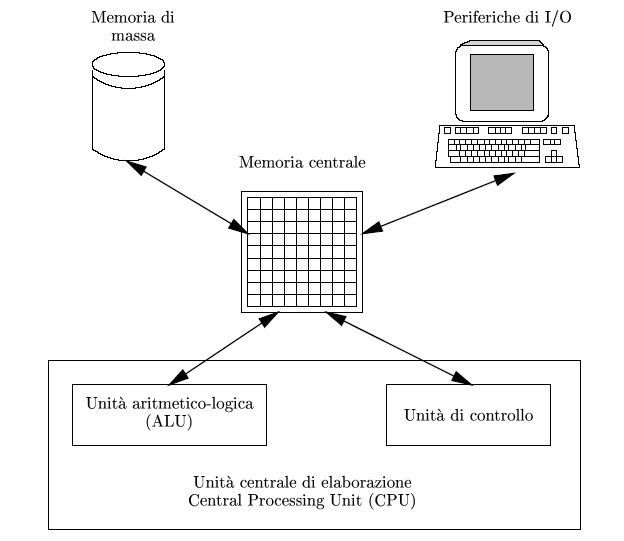
\includegraphics[scale=0.5]{von1.png}\\
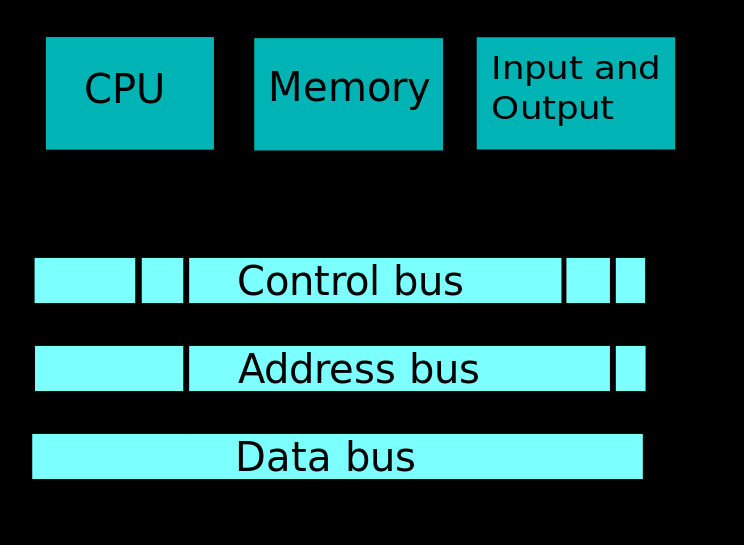
\includegraphics[scale=0.5]{von2.png}
\end{center}
\newpage
\paragraph{La scheda madre} di un computer è una scheda
formata da chip (circuiti integrati elettronici)
Contiene l'unità centrale di elaborazione (CPU), le
memorie e gli slot (prese) per le schede di
espansione con le quali possiamo collegare le
periferiche.
\paragraph{Le memorie} presenti in un computer
possono essere suddivise in: \textbf{memorie centrali} o
principali (main memory) \textbf{memorie di massa}, \textbf{memorie
esterne} (USB).\\
La capacità Le memorie possiedono una capacità che si
esprime in Byte Scala di equivalenza: 1 Byte equivale a 8
bit; 1 chilo Byte (1 KByte) equivale a 1024 Byte; 1 mega
Byte (1 MByte) equivale a 1024 KByte; 1 giga Byte (1
GByte) equivale a 1024 MByte; 1 tera Byte (1 TByte)
equivale a 1024 GByte. 1 peta Byte (1 PByte) equivale a
1024 TByte).
\paragraph{Le Memorie Centrali}
\begin{itemize}
\item Le memorie principali: Vengono anche chiamate memorie centrali Contengono
un numero limitato di informazioni. Si dividono in: memoria RAM (Random Access
Memory), cioè memoria ad accesso casuale, consente sia la scrittura che la lettura
dei dati in essa contenuti memoria ROM (Read Only Memory), cioè memoria di
sola lettura, consente soltanto la lettura dei dati in essa contenuti memoria Cache.
\item Memoria RAM: La RAM (Random Access Memory) è la memoria che contiene i
dati e i programmi in corso di esecuzione E di tipo volatile, significa che perde il
suo contenuto quando il computer viene spento.
\item Memoria ROM: La ROM (Read Only memory) è una memoria di sola lettura.
Contiene un programma che permette di accendere il computer, chiamato BIOS
(Basic Input Output System).
\item Cache memory: La memoria cache (termina che deriva dalla lingua francese e
che significa nascosto) svolge un compito di memorizzazione temporanea dei dati.
Coadiuva la CPU nella comunicazione con la memoria RAM.
\end{itemize}

\paragraph{Le Memorie di Massa} Hanno lo scopo di conservare i programmi e i dati in modo permanente. Le
memorie di massa più diffuse sono collocate all'interno del case (memorie
interne) Le memorie di massa che possono essere collegate esternamente
al computer, vengono chiamate memorie esterne.
\\Si presentano in moltissimi formati, che vanno dai meno recenti floppy disk
fino ai nuovissimi blu-ray disk. Quasi tutti sono composti da dischi estraibili,
eccezion fatta per i dischi fissi o dischi rigidi (hard disk).
\\Dischi Fissi Sono collocati all'interno del case e non sono normalmente
estraibili né visibili dall'esterno I primi modelli avevano una capacità di pochi.
MByte, mentre i modelli più attuali fino ad alcuni TByte Normalmente ogni
PC ne contiene uno solo ma è possibile aggiungerne anche qualche altro.

\paragraph{La CPU.} Durante il suo funzionamento, non fa altro che eseguire le
istruzioni di un programma Il programma è formato da istruzioni
scritte attraverso un linguaggio apposito, chiamato linguaggio
macchina, composto da istruzioni scritte in forma binaria. La
CPU è in grado di eseguire milioni di istruzioni al secondo e, in
base al tipo di istruzione, incarica altri dispositivi di eseguire
alcuni compiti.\\Se viene impartito al computer il comando di stampare un
documento, la CPU incarica la periferica di eseguire la stampa,
quindi i dati vengono letti dall'unità a disco e inviati attraverso il
bus alla periferica desiderata. L'utente effettua pertanto solo un
click e al resto penserà la CPU.

\paragraph{Architettura di un Host (Server)} Come sarà più chiaro in seguito, la parola chiave quando si tratta di strutturare un server è "ridondanza". In generale, "più componenti sono ridondanti in un server, meglio è" è un'affermazione parecchio solida.\\
A livello visivo, il server è spesso composto da un armadio (rack) nel quale possono venire installati vari moduli attraverso delle "rotaie". Questi moduli sono, ad esempio, gruppi di continuità, unità esterne di computing, e ovviamente, l'unità centrale del server.\\
Un server, proprio per il fattore di ridondanza, può avere più di un alimentatore, più di un processore, e così via.\\
Oltre a queste caratteristiche di base, è utile confrontare l'hardware di un PC con quello di un server, in quanto le componenti necessarie per far funzionare entrambi sono le stesse, ma ci sono differenze sostanziali che influiscono sul funzionamento e sulle prestazioni dei sistemi:
\begin{itemize}
\item \textbf{CPU:} i processori per server (i.e.: Intel Xeon, ecc.) sono dotati di più cores e più memoria cache, ma tendenzialmente operano a frequenze più basse rispetto ai processori consumer-grade in quanto i processi server sono ottimizzati per l'esecuzione multicore, mentre i processi più comuni per gli utenti lavorano per la maggior parte su un singolo core, e di conseguenza fanno affidamento sulla frequenza di clock del processore.
\item \textbf{RAM:} anche qui la differenza è marcata, in quanto le RAM consumer-grade (specialmente le RAM DDR4) fanno affidamento sulle frequenze alte ma sacrificando i tempi di latenza, mentre le RAM da server adottano un approccio che favorisce la latenza a scapito della frequenza. Inoltre, le RAM da server sono dotate di tecnologia ECC (error correction code), una tecnologia che permette di correggere gli errori presenti nei dati memorizzati.
\item \textbf{Dischi:} i dischi sono molto più veloci, spesso anche il doppio rispetto a quelli consumer-grade. Inoltre vengono studiati per durare più a lungo, sono dotati di una memoria cache di relativamente grandi dimensioni e vengono disposti in RAID nella quasi totalità dei casi.
\item \textbf{Schede di Rete:} di solito il PC che abbiamo a casa fa affidamento sulla scheda di rete integrata sulla scheda madre, mentre nel caso dei server solitamente si usano almeno due schede di rete dedicate con porte gigabit o fibra.
\item \textbf{Raffreddamento:} mentre nei PC consumer grade il raffreddamento è affidato a un dissipatore (ad aria o a liquido), nei server anche la sala dove sono posizionati deve essere refrigerata a causa della quantità di calore che viene sprigionata. Questo rende la sala server parecchio rumorosa.
\item \textbf{Alimentatori:} gli alimentatori per i server non solo hanno una capacità (in termini di Watt) superiore a quella che verrà effettivamente richiesta dal sistema, ma spesso un server ha più alimentatori nel caso in cui uno o più di questi falliscano (ridondanza). 
\item \textbf{Gestione remota:} esiste la possibilità di controllare remotamente il server grazie ad una tecnologia sviluppata da Hewlett-Packard, chiamata ILO (Integrated Lights Out). Fisicamente si presenta come una porta Ethernet dedicata. Le possibilità che si hanno grazie a ILO sono quelle di riavviare il server, accendere il server, montare disk images da remoto e accedere al server IML (Integrated Management Log), tutto questo grazie al fatto che la ILO è dotato di una connessione separata da quella del server.
\end{itemize}
Prima di parlare dell'organizzazione dei dischi, una piccola considerazione: per quanto possano aumentare le capacità di archiviazione dei dischi grazie all'addensarsi delle aree di memoria nei piatti, le velocità diminuiscono di pari passo. Una soluzione sarebbe quella di adottare degli SSD, ovvero delle unità a stato solido che memorizzano i dati grazie a delle porte NAND. Permettono di raggiungere velocità elevate in lettura e scrittura, ma sono meno affidabili e tendenzialmente hanno una durata di vita minore rispetto ai tradizionali hard disk.
\paragraph{RAID - Redundant Arrat of Inexpensive/Independent Disks} Il RAID non è altro che un costrutto logico (astrazione) che permette di organizzare due o più dischi in maniera tale da raggiungere migliori specifiche in termini di sicurezza, velocità e/o capacità. Questo costrutto può essere messo in atto grazie a un controller RAID, integrato nella maggior parte delle schede madri, ma per risultati migliori (specialmente in presenza di grandi quantità di dischi) si fa affidamento su controller RAID esterni collegati alla scheda madre tramite connettori PCI/E.\\
Esiste anche la possibilità di eseguire un RAID a livello software, ma in genere non viene utilizzato in quanto non è conveniente in termini di affidabilità e prestazioni. Questo è dovuto al fatto che il RAID software è un'astrazione ulteriore rispetto al RAID hardware, processo che avviene ad un livello più basso.\\
Prima di affrontare il RAID nelle sue forme principali, va precisato che questo \textbf{non} sostituisce il backup.
\begin{itemize}
\item \textbf{RAID 0:} detto anche striping, è un sistema in grado di separare i dati in singole stringhe in modo da scrivere ognuna di queste in un disco diverso. \begin{center}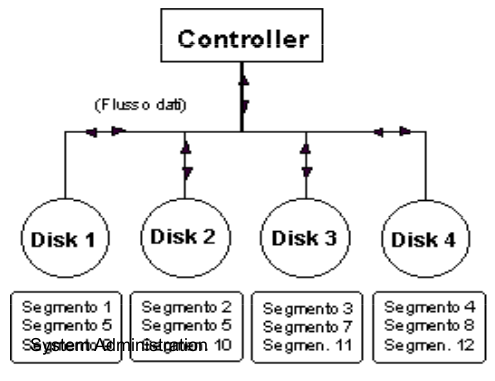
\includegraphics[scale=0.5]{raid0.png}\end{center}
Migliora la velocità in lettura in base al numero dei dischi, ma è molto rischioso in quanto basta il malfunzionamento di uno qualsiasi dei dischi e i dati vengono persi.

\item \textbf{RAID 1:} detto anche mirroring, questo tipo di RAID mantiene una duplice copia degli stessi dati in due dischi diversi. Questo comporta all'avere una maggiore velocità in lettura, ma prestazioni pessime in scrittura, in quanto i bit dei dati vengono scritti più volte. Il vantaggio è quello di avere la massima ridondanza dei dati.
Pur tenendo conto di quest'ultima caratteristica, le prestazioni ridotte lo rendono applicabile solamente nei piccoli sistemi o dov'è fondamentale la salvaguardia dei dati. \begin{center}
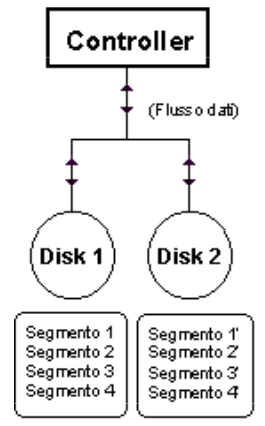
\includegraphics[scale=0.5]{raid1.png}\end{center}

\item \textbf{RAID 3} sistema simile allo striping: necessita di almeno tre dischi, ma in uno di questi vengono memorizzate le stringhe di parità, ovvero una specie di mappatura dei bit che permette la ricostruzione dei dati in caso di guasti. Questo però non permette al sistema di essere espandibile, in quanto il disco di parità non avrebbe la capienza per contenere tutte le stringhe. per espanderlo bisognerebbe cambiare tutti i dischi. Si hanno alte prestazioni in accesso a grossi files, ma letture e scritture non simultanee. \begin{center}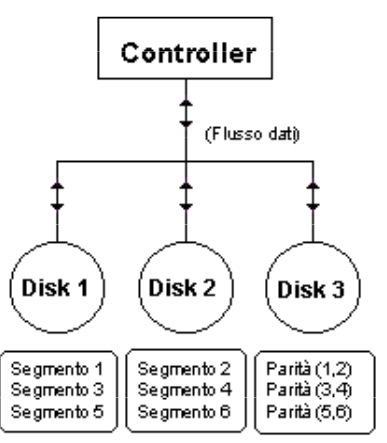
\includegraphics[scale=0.5]{raid3.png}\end{center}

\end{itemize}
\begin{itemize}
\item \textbf{RAID 5:} è un'ottimizzazione del RAID 3, dove le stringhe di parità sono salvate in modo ordinato in tutti i dischi del RAID. Necessita di almeno tre dischi (tutti della stessa dimensione), e la capacità è sempre pari a \texttt{((n-1)*C)} byte, dove \texttt{n} è il numero di dischi e \texttt{C} è la loro capacità. Questo sistema è usato nei grossi sistemi multiutenza, dove le operazioni di scrittura sono molto inferiori a quelle di lettura. Il fault tolerance è pari a 1, ovvero il sistema funziona anche se un disco fallisce. \begin{center}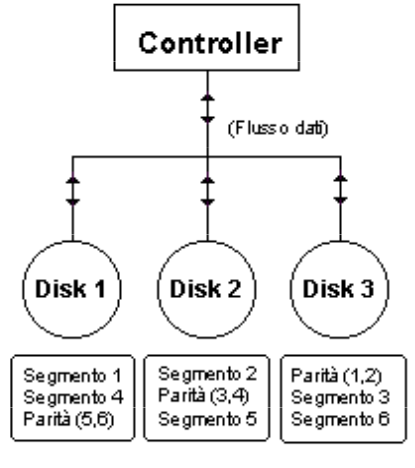
\includegraphics[scale=0.5]{raid5.png}\end{center}

\item \textbf{RAID 6:} questo sistema usa una divisione a livello di blocchi con i dati di parità distribuiti due volte tra tutti i dischi. Non era presente tra i livelli RAID originari. Nel RAID 6, il blocco di parità viene generato e distribuito tra due stripe di parità, su due dischi separati, usando differenti stripe di parità nelle due direzioni. Il RAID 6 è più ridondante del RAID 5, ma è molto inefficiente quando viene usato in un numero limitato di dischi.

\item \textbf{RAID 7:} il RAID 7 è un tipo di RAID proprietario che aggiunge un sistema di caching ai RAID 3 o 4.

\item \textbf{RAID 1+0:} sistema in grado di rigenerare i dati anche in presenza di rotture in più dischi, mantenendo buone prestazioni (migliori rispetto ai raid 5 e 6 in quanto non devono venire gestite le informazioni di parità). Rimane un RAID molto costoso, in quanto la capacità complessiva dei dischi va sempre dimezzata, e l'espansione del sistema va effettuata con coppie di dischi uguali. Necessita di almeno quattro dischi per essere messo in atto. Viene impiegato in grossi sistemi dove si necessita di velocità massima e una sicurezza dati di alto livello. \begin{center}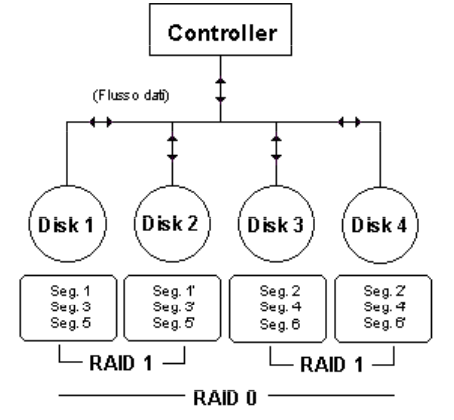
\includegraphics[scale=0.5]{raid1+0.png}\end{center}

\end{itemize}

\chapter{Network Attached Storage - NAS}
In una rete aziendale la flessibilità è molto importante: poter
espandere la capacità di storage al crescere della rete senza
però intervenire sui dispositivi già installati può essere un
problema.
\\Fino a 10 anni fa era necessario acquistare nuovi server da
aggiungere alla rete o in sostituzione di altri solo per avere più
storage: DAS (Direct Attacched Storage) o SAS (Server
Attacched Storage).
\\Ora tramite la tecnologia NAS si possono aggiungere dispositivi
con grosse capacità di storage (e spesso scarse di calcolo) che
garantiscono scalabilità nel tempo a costi contenuti.
Il NAS è un computer (host) con:
\begin{itemize}
\item Almeno una CPU
\item Una scheda madre
\item \texttt{N} hard disk in raid (1,1+0,5,6 ecc)
\item \texttt{K} SSD da utilizzare come cache (Sinology)
\item Un sistema operativo (Linux based, solitamente)
\item \texttt{M} schede di rete veloci (almeno 1Gbs)
\end{itemize}
\paragraph{Quali sono gli utilizzi del NAS?}
\begin{itemize}
\item Si utilizza come storage per le home utenti .
\item Si utilizza come storage per i backup.
\item Si utilizza come storage per le macchine virtuali.
\item Si utilizza come storage per database, siti web ecc.
\end{itemize}
Insomma è uno storage, ma va pesato a seconda degli usi e
possibilmente rindondato.\\
Un NAS può contenere più volumi, che possono essere
replicati su altri NAS e visibili solo da chi si vuole (tramite ACL).\\
La formula RAID + Rindondanza NON sostituisce il backup.\\
\chapter{Storage Area Network - SAN}
Il SAN è una soluzione altamente professionale adottata da quasi tutte le grosse compagnie (meno popolari nelle medie dimensioni) per fronteggiare le necessità di storage. Il ruolo del SAN è quello di sostituire quelli che sono i sistemi più tradizionali, come ad esempio DAS (Directly Attached Storage) o SAS (Server Attached Storage). In sostanza, consiste in una LAN dedicata unicamente allo storage, affiancata alle LAN aziendali per non impattare sulle loro prestazioni. \\
Il vantaggio rispetto ai sistemi tradizionali è particolarmente evidente se si opera un confronto tra questi e il SAN.\\
Tradizionalmente, vengono utilizzati dispositivi collegati direttamente ai server che condividono le informazioni sulla LAN. Questo sistema presenta dei limiti:
\begin{itemize}
\item Gestione dell'accesso alle informazioni complicata.
\item La rete è un collo di bottiglia (1000MBit).
\item I server sono un collo di bottiglia.
\item Il formato dei dati è vincolato al sistema a cui è connesso il device.
\item Le prestazioni dei server e dei devices non sono pienamente
sfruttate.
\item Degrado delle prestazioni della rete.
\item Inefficienza crescente al crescere delle richieste e degli utenti.
\item Spreco di banda, CPU e RAM: ogni trasferimento implica la
negoziazione di parametri per la connessione.
\end{itemize}
Il SAN, invece:
\begin{itemize}
\item Architettura scalare che si adatta bene alle
evoluzioni di una azienda.
\item Permette di collocare le risorse dove servono.
\item Sono il risultato di un buon lavoro di
progettazione.
\item Permettono la scalabilità in termini di storage,
banda e connettività senza interruzione dei
servizi.
\end{itemize}
Il fattore della dislocazione geografica è da tener conto: infatti, se un'azienda ha più edifici il SAN si può applicare con un collegamento in fibra ottica se gli edifici sono in un raggio di 10km, con protocolli di Storage Over IP altrimenti.

\chapter{Canali di Trasmissione}
Mezzo o canale trasmissivo è il supporto fisico
tramite il quale un segnale si propaga da un
punto ad un altro di una rete.\\
Quando si mettono in collegamento due
interlocutori si dice che fra questi si stabilisce un
canale di comunicazione.\\
Su un mezzo trasmissivo vi possono essere
simultaneamente più canali e un canale può
usare più mezzi trasmissivi.\\
I mezzi e canali di trasmissione sono così classificati:
\begin{itemize}
\item \textbf{Mezzi di trasmissione:}
	\begin{itemize}
	\item doppino telefonico
	\item cavo coassiale
	\item fibra ottica
	\item etere (wi-fi)
	\end{itemize}
\item \textbf{Canali}
	\begin{itemize}
	\item simplex: flusso dati unidirezionale
	\item half-duplex: flusso alternativo nelle 2 direzioni
	\item full-duplex: flusso simultaneo nelle 2 direzioni
	\item punto-punto e multi-punto
	\end{itemize}
\end{itemize}
I parametri rilevanti quando si parla di mezzi o canali di trasmissione sono i seguenti:
\begin{itemize}
\item \textbf{Velocità di trasmissione}
	\begin{itemize}
	\item i dati sono codificati in bit
	\item si misura in bps (bit per secondo) o con i suoi multipli Kbps (kilobit per secondo) e Mbps (megabit per secondo) e così via
	\end{itemize}
\item \textbf{Larghezza di banda}
	\begin{itemize}
	\item indica la massima capacità trasmissiva di un mezzo
	\item si misura anch'essa con le unità di misura indicate in precedenza
	\end{itemize}
\end{itemize}
\paragraph{Confronto banda/velocità:} su un mezzo trasmissivo possono essere realizzati più canali che "dividono" la banda; pur avendo allora un'elevata larghezza di banda, ciascun canale avrà una ridotta velocità di trasmissione.
\paragraph{Doppino telefonico (rame):} è costituito da due a otto sottili fili di rame intrecciati, e il suo utilizzo varia da rete a rete, ognuna delle quali hanno categorie diverse di cavo, che definiscono la banda massima garantita. Inoltre, più si sale di categoria, maggiori sono le proprietà che acquisisce il cavo, come il miglioramento della qualità costruttiva, la minor perdita di segnale, ecc..
\paragraph{Fibra ottica:} è costituita da decine o centinaia di sottili fibre di vetro o di
materiale plastico che trasmettono impulsi di luce.
\\Già utilizzata per le dorsali oceaniche e per le LAN ad alta
velocità. Un sistema di trasmissione su fibra ottica consiste di una
sorgente luminosa, del mezzo di trasmissione e di un ricevitore; la
sorgente luminosa converte segnali elettrici in impulsi per poi
riconvertirli in segnali elettrici alla fine del tragitto. Diciamo pure
che un segnale luminoso rappresenta il bit a 1 e l'assenza di luce
rappresenta il bit a 0.
\\La fibra ottica necessita di ripetitori, per via dell'attenuazione del
segnale, ogni 50km rispetto i 5km del doppino, non è affetta da
disturbi esterni e ha una capacità di trasmissione molto elevata.
\paragraph{WiFi:} viene usato l'etere come mezzo trasmissivo e
consentono di creare facilmente reti senza
installare alcun tipo di cablaggio, operazione in
molti casi costosa.
\\Si utilizza un apparecchio, detto access point,
collegato fisicamente alla rete, che comunica
con gli utenti attraverso segnali radio. I computer
degli utenti devono essere dotati di una scheda
per il collegamento wireless, detta scheda wi-fi.

\chapter{Networking}
In alcune situazioni l'amministratore di sistema deve essere anche un po’
amministratore di rete: ad esempio nelle piccole aziende i due ruoli
coincidono.\\
Le reti possono essere classificate in tre categorie:
\begin{itemize}
\item \textbf{LAN o Local Area Network:} identifica una rete costituita da computer
collegati tra loro, dalle interconnessioni e dalle periferiche condivise in un
ambito fisico delimitato
\item \textbf{MAN o Metropolitan Area Network:} è una rete dati che interconnette
un'area corrispondente a quella di una grande città. Le reti di questo tipo
vengono realizzate con tecniche innovative come, per esempio, la posa di cavi
a fibre ottiche o la tecnologia wireless. Una MAN può interconnettere tra loro
diverse LAN
\item \textbf{WAN o Wide Area Network:} indica in generale una rete di grande
estensione, e a cui in genere si fa riferimento per indicare la struttura che
connette varie reti locali, estendendosi potenzialmente su tutto il mondo
(Internet è un esempio di WAN)
\end{itemize}
\paragraph{Il protocollo TCP/IP:}
per protocollo si intende un insieme di regole che delineano il formato che deve essere utilizzato nella
comunicazione tra due sistemi.\\
Il TCP/IP Internet Protocol Suite è il nome dato ad un set di protocolli sviluppato in seno al
DoD degli Stati Uniti (Department of Defense) dal DARPA (Defense Advanced Research
Project Agency). \\All'epoca esisteva una sola rete, ARPA-net, che connetteva solo pochi
computer a livello universitario.
I dati, per transitare su di una rete, devono essere divisi in piccoli pezzi, ognuno dei quali
viene inviato separatamente. Su di una rete IP, questi pezzetti sono chiamati "pacchetti";
tutti i trasferimenti di dati avvengono sotto forma di pacchetti.Il protocollo TCP/IP è costruito
con un modello a strati, in cui le informazioni si fanno strada da un'applicazione su un host
ad un'applicazione su un altro host attraverso varie trasformazioni (incapsulamenti,
frammentazione, ecc).
\\In una rete TCP/IP ogni host è identificato da un indirizzo IP univoco all'interno di essa.
Non rispecchia lo schema standard ISO/OSI per la scrittura corretta di un protocollo di
comunicazione ma 
è scritto talmente bene ed è talmente semplice da essere sempre efficiente.\\
\begin{center}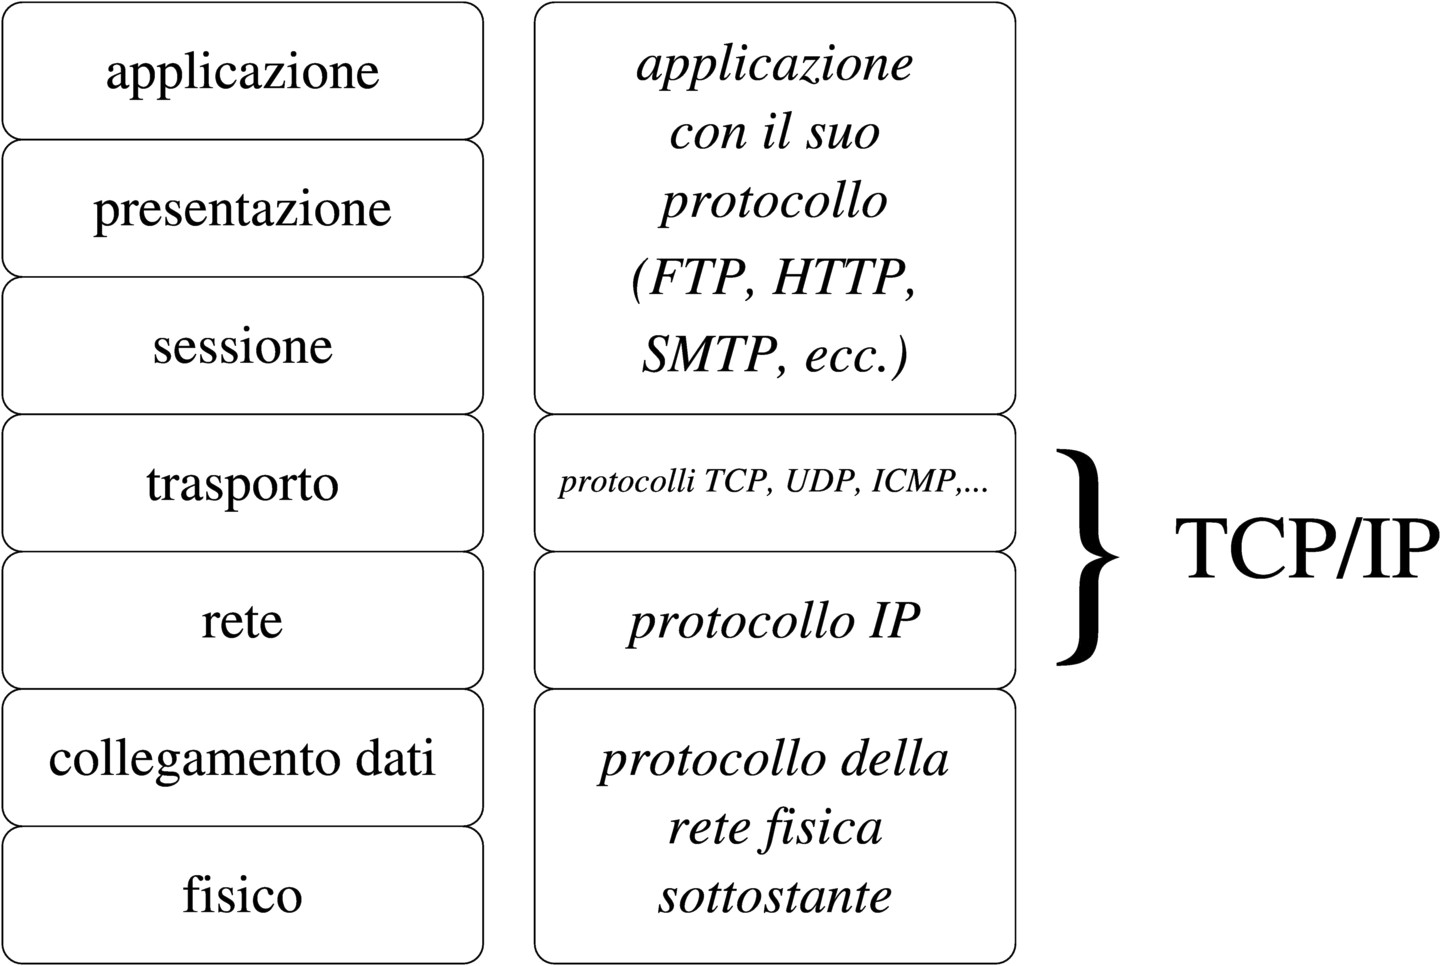
\includegraphics[scale=0.25]{tcpip.png}\end{center}
\begin{center}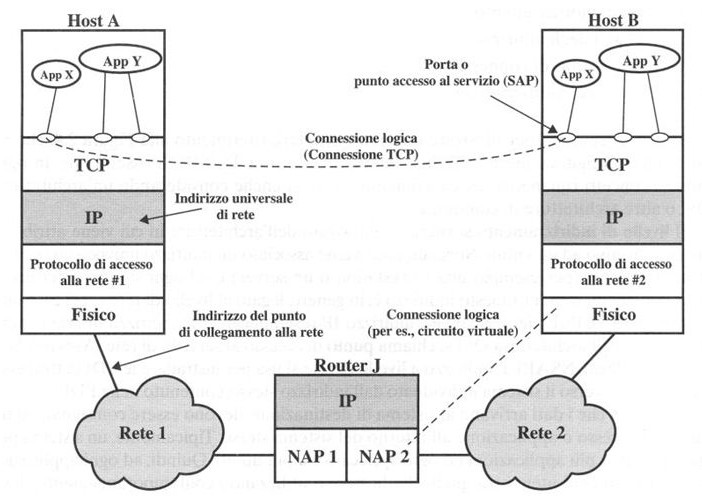
\includegraphics[scale=0.5]{tcpip2.png}\end{center}
I dispositivi che compongono la struttura di un network sono i seguenti:
\begin{itemize}
\item \textbf{Router:} si occupa di instradare I pacchetti in/out rispetto alla
LAN. Spesso è uno switch evoluto.
\item \textbf{Hub:} inoltra I pacchetti su tutte le porte la velocità viene
condivisa e si presentano collisioni.
\item \textbf{Switch:} mantiene una tabella di corrispondenza tra porte e mac
address delle schede di rete ad esse collegate. In tal modo
instrada I pacchetti direttamente alla scheda di rete corretta,
evitando collisioni e garantendo sempre la velocità massima.
\item \textbf{Access point:} permette accesso alla rete tramite connessione
wifi (è un po' router e un po' switch).
\end{itemize}
È interessante notare come in un semplice network casalingo alcuni di questi componenti sono presenti in un unico dispositivo, mentre in una rete di un certo spessore ogni dispositivo ha il suo compito.\\
\paragraph{IPv4:} ogni qualvolta un dispositivo si connette a un network, gli viene assegnato un indirizzo IP. Gli indirizzi IP versione 4, , sono composti da una sequenza
di 32 bit, suddivisi convenzionalmente in quattro gruppi di 8
bit, e rappresentati in modo decimale separati da un punto.\\
All'interno di un indirizzo del genere si distinguono due parti:
l'indirizzo di rete e l'indirizzo indirizzo del nodo particolare.
Il meccanismo utilizzato per distinguere la parte dell'indirizzo
che identifica la rete è quello della maschera di rete o
netmask.\\
La maschera di rete è un indirizzo che viene abbinato
all'indirizzo IP da analizzare con l'operatore booleano AND,
per filtrare la parte di bit che interessano.\\
\paragraph{Classi di indirizzi IPv4:}
\begin{itemize}
\item \textbf{Indirizzi di classe A:} Il valore del primo ottetto è compreso tra 1 e 126. E' rappresentata da
indirizzi di tipo: \texttt{Rete.Host.Host.Host} ovvero 8 bit per la identificare la rete (di cui il primo fisso) e
24 per identificare gli host. Permette di ottenere 126 reti formate da 16.774.214 host ciascuna.
\item \textbf{Indirizzi di classe B:} Il valore del primo ottetto è compreso tra 128 e 191. E' rappresentata da
indirizzi di tipo: \texttt{Rete.Rete.Host.Host} ovvero 16 bit per la identificare la rete(di cui i primi due
fissi) e 16 per identificare gli host. E' possibile ottenere 16.384 reti formate da 65.534 host
ciascuna.
\item \textbf{Indirizzi di classe C:} Il valore del primo ottetto è compreso tra 192 e 223. E' rappresentata da
indirizzi di tipo: \texttt{Rete.Rete.Rete.Host} ovvero 24 bit per la identificare la rete (di cui i primi tre
fissi) e 8 per identificare gli host. E' possibile ottenere 2.097.152 reti con 254 host ciascuna.
\item \textbf{Indirizzi di classe D:} Il valore del primo ottetto è compreso tra 224 e 239. Sono indirizzi di rete
riservati ai gruppi multicast e non assegnabili ai singoli host.
\item \textbf{Indirizzi di classe E:} Il valore del primo ottetto è compreso tra 240 e 255. Sono indirizzi
riservati per usi futuri.
\end{itemize}
\begin{center}
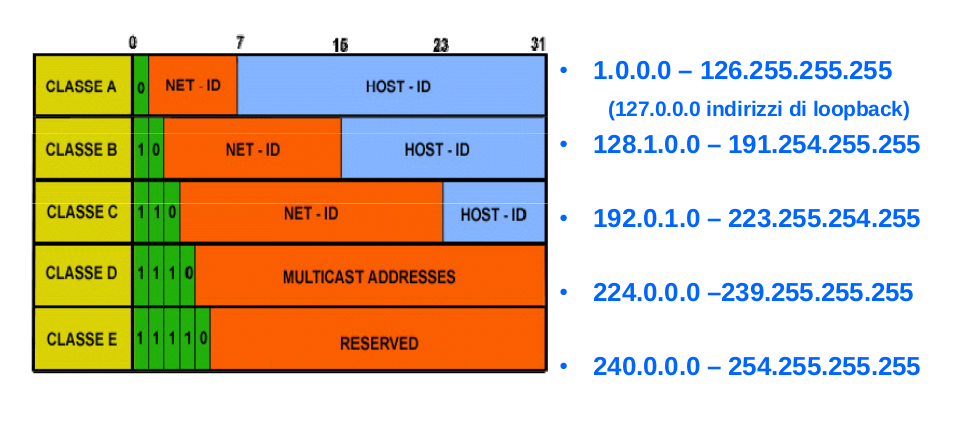
\includegraphics[scale=0.5]{ipv4classi.png}
\end{center}
Esistono, infine, degli indirizzi "speciali":
\begin{itemize}
\item \texttt{0.0.0.0}: default route
\item \texttt{127.0.0.1}: loopback
\item Range classe A: \texttt{10.0.0.0} - \texttt{10.255.255.255}
\item Range classe B: \texttt{172.16.0.0} - \texttt{172.31.255.255}
\item Range classe C: \texttt{192.168.0.0} - \texttt{192.168.255.255}
\end{itemize}
Esistono due notazioni principali attraverso le quali è possibile indicare un indirizzo IP:
\begin{itemize}
\item \textbf{Indicando espressamente la subnet mask:}
	\begin{itemize}
	\item \texttt{49.22.5.3 255.0.0.0} - Classe A;
	\item \texttt{172.16.20.5 255.255.0.0} - Classe B;
	\item \texttt{192.168.15.4 255.255.255.0} - Classe C;
	\end{itemize}
\item \textbf{Indicando i bit che compongono la subnet mask:}
	\begin{itemize}
	\item \texttt{49.22.5.3/8} - Classe A;
	\item \texttt{172.16.20.5/16} - Classe B;
	\item \texttt{192.168.15.4/24} - Classe C;
	\end{itemize}
\end{itemize}
Alcune classi di indirizzi, definite nella RFC
1918, vengono chiamati privati e sono utilizzati
per le reti locali non connesse ad internet:
\begin{itemize}
\item Da \texttt{10.0.0.0.0} a \texttt{10.255.255.255.255}
\item Da \texttt{172.16.0.0} a \texttt{172.31.255.255}
\item Da \texttt{192.168.0.0} a \texttt{192.168.255.255}
\end{itemize}
\paragraph{Approfondimento sugli indirizzi speciali.} Esistono alcuni particolari indirizzi di rete che non possono essere assegnati per
l'identificazione di un host, tra questi abbiamo: network e broadcast e loopback:
\begin{itemize}
\item \textbf{Network:} quando i bit dell'ottetto che rappresenta l'host hanno tutti valore 0,
l'indirizzo è detto di rete o Network Address: \texttt{192.168.5.0}
\item \textbf{\texttt{0.0.0.0:}} quando tutti i bit hanno valore zero, identificano "questo host";
\item \textbf{Broadcast:} quando i bit del numero che rappresenta l'host hanno tutti valore 1,
l'indirizzo è detto di broadcast o broadcast address, e rappresenta tutti gli host di
quella rete. Inviare un pacchetto all'indirizzo \texttt{192.168.5.255} equivale a mandare un
pacchetto a tutti gli host della rete \texttt{192.168.5.0};
\item \textbf{Broadcast di rete:} abbiamo questo tipo di indirizzo quando tutti i bit, sia della parte
relativa all'host sia della parte relativa alla rete hanno valore 1. Inviare un pacchetto
a \texttt{255.255.255.255} significa inoltrarlo verso tutti gli host della rete corrente;
\item \textbf{Loopback:} è utilizzato per funzioni di test del protocollo TCP/IP, non genera traffico
di rete e corrisponde all'indirizzo \texttt{127.0.0.1};
\end{itemize}
La struttura della codifica degli indirizzi IPv4 permette di avere un certo numero limitato di indirizzi IP codificabili. Questi indirizzi vengono assegnati a blocchi agli ISP, e ora sono finiti. È nata quindi l'esigenza di avere un nuovo formato di indirizzi IP, che permetta di codificare più unità.\\
Nascono quindi gli indirizzi \textbf{IPv6}.\\
Il nuovo formato dell'IP, ora di 128 bit a fronte
dei 32 della precedente versione (IPv4), porta in
sé notevoli cambiamenti che dovranno essere
affrontati dall'intera utenza web.\\
Prima di IPv6 venne sperimentato il protocollo IPv5, che venne però abbandonato.\\
IPv6 usa indirizzi 4 volte più lunghi di quelli IPv4. IPv4 ha un
massimo teorico di circa 4 miliardi di indirizzi, mentre IPv6 ha un
massimo teorico di circa 340 miliardi di miliardi di miliardi di
miliardi. Siccome gli indirizzi IPv6, come già quelli IPv4, devono
essere strutturati per il routing e per altri scopi, il numero di indirizzi
realmente utilizzabili è minore, ma sempre estremamente grande.\\
Un tipico indirizzo IPv6 è composto da 8 gruppi
separati dal carattere “:”. Ogni gruppo è composto
da un massimo di quattro lettere e numeri, come
può essere \texttt{2001:db8:1f70:999:de8:7648:6e8:1}.\\
\begin{center}
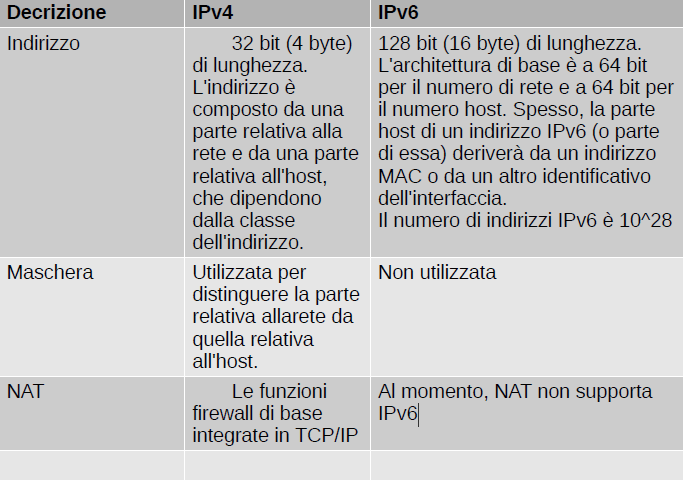
\includegraphics[scale=0.65]{ipv4vsipv6.png}
\end{center}
IPv4 è sopravvissuto fin'ora grazie al NAT che
permette di convertire indirizzi di rete privati in
un unico indirizzo di rete pubblico. (definzione
molto approssimativa).\\
Perché, però, non passiamo direttamente agli indirizzi IPv6? \\
Per la stessa regola enunciata all'inizio del documento: perché cambiare un sistema che funziona?\\
Perché ad esempio un firewall con \texttt{iptables} (che
vedremo) configurato per IPv4 viene totalmente
bypassato da IPv6.\\
Perché significa dover adeguare apparati,
sistemi operativi, host e personal computer e
cambiare regole e politiche di sicurezza interne.

\chapter{Filesystems}
I filesystems sono la parte del sistema operativo che si occupa della gestione dei files, formattando opportunamente le unità di memoria di massa, registrando e leggendo i files.\\
Viene visto in modi differenti:
\begin{itemize}
\item \textbf{Utente:} appare come un insieme di file e directory
ed è usato per memorizzare e organizzare i dati in
modo che siano accessibili al sistema e ai suoi
utenti.
\item \textbf{OS:} è un insieme di strutture di controllo e blocchi
di dati che occupano uno spazio ben definito da
una partizione (porzione del disco) che permette di
memorizzare e gestire i dati.
\end{itemize}
Che cos'è realmente un file? Un file non è altro che un'astrazione del sistema operativo che permette di usare in modo semplice ed efficiente i dispositivi di memoria secondaria. \\
Ogni file possiede attributi (nome, tipo, dimensione,
protezione, data, ora ecc).
I file possono essere creati, letti, scritti, cancellati ecc..
I nomi dei file possono avere, nei SO moderni una
lunghezza compresa tra 1 e 255 caratteri (percorso
compreso).\\

Esistono vari tipi di files:
\begin{itemize}
\item File regolari (o file utente, sono \texttt{ASCII} o \texttt{BIN})
\item Directory (contengono file regolari e non in una
struttura gerarchica)
\item File speciali a blocchi (unità di I/O a blocchi).
\item File speciali a caratteri (unità di I/O a caratteri).
\item I file si distinguono per le estensioni: \texttt{exe, jpg, gif,
mov, mkv, ecc.}
\item In windows un file speciale è quello di \texttt{Swap}
\end{itemize}
\paragraph{Directory:} è un elenco di nomi di file (o/e altre directory) a cui
è associato un nome. Fondamentale per dare una struttura gerarchica al
filesystem. In una struttura ad albero la radice è detta radice
del filesystem (/ o c:\textbackslash). Sulle directory si possono effettuare le seguenti
operazioni: creazione, cancellazione, link, unlink,
rename ecc..
\begin{center}
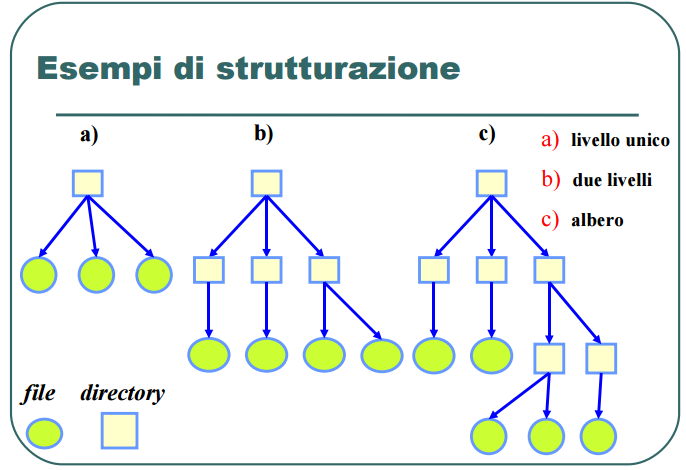
\includegraphics[scale=0.5]{strutturadir.png}
\end{center}
\paragraph{Struttura di un Filesystem in Linux/Unix}
\begin{itemize}
\item \texttt{/etc}, directory che contiene, tipicamente, i file di configurazione del sistema.
\item \texttt{/bin}, che contiene alcuni programmi essenziali.
\item \texttt{/sbin}, che contiene alcuni programmi essenziali che tipicamente l'utente
comune non deve lanciare autonomamente.
\item \texttt{/lib} che contiene le librerie dinamiche necessarie ai programmi delle due
directory precedenti.
\item \texttt{/usr}, che contiene tutti i programmi che non sono necessari nelle prime fasi di
avvio del sistema, nonché le relative librerie e file accessori, nelle directory
\texttt{/usr/[s]bin,/usr/lib} e \texttt{/usr/share}, rispettivamente
\item \texttt{/usr/local}, che dispone anche di sotto-directory simili a quelle di \texttt{/usr}, in cui
vengono memorizzati programmi e librerie installati dall'amministratore e scelti
al di fuori di quelli forniti dalla distribuzione. Funzione simile ha \texttt{/opt}, che viene
usato per quei programmi che non rispettano la convenzione di separazione
dei binari dalle librerie e dai file accessori.
\item \texttt{/home}, contiene gli spazi di memorizzazione personali (home directory)
degli utenti.
\item \texttt{/root}, è la home directory dell'utente root.
\item \texttt{/var}, contiene i dati di tutte quelle applicazioni di uso generale del sistema, e
non del singolo utente. Qui dentro vi sono, tipicamente, i dati relativi ai
server (software) che forniscono i vari servizi. Di particolare importanza la
directory \texttt{/var/log}, che contiene i log (registri degli eventi) del sistema,
gestiti direttamente dalle relative applicazioni o dal servizio syslog.
\item \texttt{/proc},
\item \texttt{/dev}, contiene file che rappresentano i dispositivi presenti nel sistema, come
ad esempio dischi e terminali.
\item \texttt{/tmp} e \texttt{/var/tmp} servono a memorizzare file temporanei.
\end{itemize}
Alcune directories più recenti aggiunte al Filesystem Linux sono:
\begin{itemize}
\item \texttt{/boot}, che contiene alcuni dei file necessari al gestore d'avvio (boot loader), nonché
il kernel ed alcuni file di supporto.
\item \texttt{/proc}, contiene dei file (o directory) che rappresentano i processi in esecuzione nel
sistema: contiene una directory per ogni processo in esecuzione, e altri file che
rappresentano lo stato del sistema. Ad esempio il file \texttt{/proc/cpuinfo} contiene
informazioni sui processori presenti nel sistema, mentre la directory \texttt{/proc/sys}.
contiene directory e file con cui è possibile modificare alcuni parametri del sistema
operativo a tempo d'esecuzione (equivalentemente al comando sysctl).
\item \texttt{/sys}, si occupa di rappresentare altre configurazioni a tempo d'esecuzione di alcuni
aspetti del sistema collegati all'hardware. Possiede una struttura più regolare
rispetto a /proc.
\item \texttt{/run} si occupa di mantenere alcuni piccoli file di stato delle applicazioni di sistema
che, sebbene siano necessarie anche per la cooperazione tra queste, non è
necessario mantenere tra i riavvii. Tradizionalmente questo compito era assolto
dalla directory \texttt{/var/run}.
\end{itemize}
Ecco un elenco dei Filesystems più conosciuti:
\begin{itemize}
\item DOS e DOSLike (Windows 95/98/Me): FAT,
FAT16, FAT32.
\item Windows NT,2000,...,2016: NTFS e le sue
evoluzioni.
\item Linux: minix, ext2, ext3, ext4, reiserFS, XFS,
UFS, ZFS, JFS.
\item MAC OS X: HFS, HFS+, APFS.
\item Novell Netware.
\end{itemize}
Uno dei Filesystems più iconici è il FAT32:
\begin{itemize}
\item Ultimo sviluppo della vecchia FAT.
\item Si basa sulla tabella FAT(File Allocation Table).
\item Facilità di creare driver che lo ha portato ad essere
l'unico filesystem che gira su tutti i sistemi (compresi i
vecchi DOS).
\item Ormai lo trovate solo sulle chiavette.
\item Poco affidabile, lento e frammentario (caro vecchio
defrag…).
\item Per sicurezza la FAT è replicata in più zone del disco.
\end{itemize}
Visti i grandi svantaggi che presentava il FAT32, si è passati all'NTFS, filesystem sviluppato da Microsoft per tutti i sistemi da Windows NT in poi.
Eccone alcune specifiche:
\begin{itemize}
\item Permette di gestire 4 miliardi di file e si basa su una tabella
chiamata MFT (Master File Table).
\item Rimane lento e obsoleto.
\item Comunque sicuro, stabile e flessibile.
\item Per sicurezza la MFT è replicata in più zone del disco.
\end{itemize}
Il filesystem di default per i sistemi Linux più recenti è Ext4, una versione migliorata di ext2. È un filesystem Journaled, veloce e performante anche per grandi quantità di piccoli files, ed è retrocompatibile con le versioni precedenti del filesystem.\\
Per i sistemi Apple, invece, il filesystem principale è HFS+, una versione Journaled di HFS. Rimane un filesystem vecchio e obsoleto, poco performante ma integrato alla perfezione con il sistema operativo, che ne copre i difetti. È stabile e affidabile, ma quest'ultima caratteristica viene meno con l'aumentare del "peso" del sistema operativo.\\
Tutto sto "journaled"... Ma cos'è? Il \textbf{journaling} è una tecnica utilizzata dai filesystems per preservare l'integrità dei dati da eventuali cadute di tensione. Ogni modifica ai dati, infatti, viene scritta in un file di log e solo secondariamente scritta sul disco.\\

Poiché i sistemi ispirati ad UNIX hanno una singola gerarchia di memorizzazione, non esiste il concetto di lettera di unità come
nei sistemi Windows. L'estensione della capacità del file system avviene perciò tramite un'operazione detta montaggio (comando
mount, file di configurazione \texttt{/etc/fstab}), in cui il file system di un'unità viene innestato in una directory del sistema. Ad esempio
la directory \texttt{/home}, con tutte le sue sotto-directory, potrebbe risiedere su un disco (o una partizione) a sé stante. Per verificare
quando spazio disco è occupato sui vari file system montati, si può usare il comando \texttt{df}.\\
Quando inserite una chiavetta USB in un sistema Linux, ad esempio Ubuntu, il sistema monta
automaticamente il volume presente sulla chiavetta in una directory temporanea:\\
\tab\texttt{\$ mount
/dev/sdd1 on /media/pippo/FedoraWSLive2513
type iso9660\\\tab(ro,nosuid,nodev,relatime,uid=1000,gid=1000,iocharset=utf8,mode\\\tab=0400,dmode=05
00,uhelper=udisk}\\
Come si crea, quindi, un filesystem in Linux/Unix?\\
Per creare un file system (nella seconda accezione descritta sopra, ovvero
un'organizzazione fisica dei dati su disco) si ricorre ai comandi della famiglia \texttt{mkfs.*} sul
device file appropriato. Si noti che solitamente, quest'ultimo, non indica l'intero disco,
ma piuttosto una partizione o, con una gestione più sofisticata, un volume logico.\\
\tab\texttt{\# mkfs.ext4 /dev/sdd1}\\
\tab\texttt{\# mkfs.ntfs /dev/sda1}\\

Per creare partizioni su disco si possono usare, a seconda del tipo di partizionamento,
\texttt{[c]fdisk} o \texttt{[g]parted.}\\
La gestione dei volumi logici e dei sottostanti gruppi di volumi e volumi fisici tramite lvm
è più complessa, e la loro trattazione richiederebbe troppo tempo, ma è generalmente
consigliata, sopratutto in ambito server dove può capitare di dover ridimensionare al
volo porzioni del disco.


\chapter{Boot di un Sistema Operativo}
\paragraph{BIOS:} è un programma scritto in una memoria
permanente (una volta erano ROM poi EPROM, poi
EEPROM) e controlla la prima fase del processo di
avvio:
\begin{itemize}
\item Effettua un test del sistema (ad esempio un blando
memtest), cerca e controlla le varie periferiche, ed
infine cerca una unità di massa da cui avviare il
sistema (hd, usb pen, dvd ecc).
\item In particolare cerca un MBR (master boot record) di
solito memorizzato nel primo settore, ne carica il
contenuto in memoria e gli passa il controllo delle
operazioni.
\end{itemize}
\paragraph{UEFI:} supera le limitazioni del vecchio BIOS consentendo, tra l'altro il boot da dischi particolarmente capienti (di capacità superiore ai 2 Terabytes) utilizzando GPT (GUID Partition Table). GPT è parte integrante dello standard
UEFI e porta con sé tutta una serie di novità rispetto all'utilizzo del MBR
(Master Boot Record).\\
Ecco alcuni vantaggi di GPT:
\begin{itemize}
\item architettura indipendente da CPU e driver.
\item ambiente preOS (accessibile cioè all'infuori del sistema operativo, prima della fase di
boot di quest'ultimo) molto più completo e versatile rispetto al passato. Si pensi che di
solito UEFI offre anche il supporto della connettività di rete.
\item design modulare.
\item eliminazione della necessità di un bootloader (fatta eccezione per utilizzi più avanzati).
\item esecuzione di moduli firmati (funzionalità Secure Boot).
\end{itemize}
MBR, o Master Boot Record, è una tabella di partizioni che cerca la prima partizione (porzione del disco) attiva (con flag di boot = 1). MBR legge il record di avvio che contiene le istruzioni su come caricare il boot loader per avviare il sistema operativo; successivamente carica il boot loader che assume il controllo del processo di avvio.\\
\paragraph{Il Boot di Windows:} il processo di boot loader viene svolto dal file NTLDR che
controlla il processo di selezione del sistema operativo e il
rilevamento dell'hardware prima dell'inizializzazione del kernel. NTLDR (il boot loader di Windows) può visualizzare un menu da cui si può
selezionare il sistema operativo operativo. La videata è
basata sulle informazioni che si trovano nel file \texttt{boot.ini}, un semplice file di testo nascosto e in sola lettura.\\
\paragraph{Il Boot di Linux:} Linux ha a disposizione tre bootloader (principali):
\begin{itemize}
\item LiLO (LinuxLoader)
\item GRUB
\item LoadLin
\end{itemize}
\paragraph{LiLO:} è il kernel loader di Linux
ed è composto da due parti: una avviabile e
una che provvede ad installarlo. La parte che
provvede ad installare LilO si appoggia sul file
\texttt{lilo.conf}.
\paragraph{GRUB:} il GRand Unified Bootloader è il bootloader più gettonato da chiunque installi un sistema operativo Linux based. Graficamente si presenta come un menù da quale scegliere che sistema operativo avviare. \\
In generale, GRUB si configura tramite un file presente in \texttt{/boot/grub} di nome \texttt{menu.lst}. Per installare GRUB, basta usare il comando \\
\tab\texttt{\#grub-install /dev/sda}\\
Su Ubuntu è un po' diverso: trovate le opzioni di default nel file \texttt{/etc/default/grub}. Altre configurazioni le trovate in \texttt{/etc/grub.d/}. Qui trovate diversi files, simili a script, che potete disattivare semplicemente togliendo i permessi di esecuzione. Per fissare le modifiche, usate il comando\\
\tab\texttt{\#update-grub}\\

\paragraph{Caricamento del kernel:} dopo aver scelto un’opzione del boot loader il
sistema carica in memoria il kernel del sistema
operativo. Il kernel si occupa di controllare che periferiche
ci sono nel computer, carica i driver relativi,
effettua delle operazioni di check preliminari,
riconosce le partizioni e cede il controllo al
processo di init. è il primo processo che il kernel manda in esecuzione dopo che il computer ha terminato la fase di bootstrap. Esso ha il compito di portare il sistema in uno stato operativo, avviando i programmi e servizi necessari.
Dato che init è sempre il primo processo eseguito, esso ha tipicamente il PID 1.
\paragraph{Init e Runlevel.} Runlevel è un particolare configurazione software del sistema
che permette l'esistenza di un solo gruppo di processi: è uno
stato del sistema che permette solo determinate azioni. Vi sono sette runlevel, numerati da 0 a 6. Generalmente quando siete in idle su ubuntu, siete in runlevel 5, 3 se non è stata caricata l'interfaccia grafica.\\
Da root potete cambiare runlevel con il comando init e
controllare in che livello siete con il comando runlevel:\\
\tab\texttt{\#runlevel}\\
\tab\texttt{\#init 3} - passa a runlevel 3\\
\paragraph{Processo di init:} \texttt{SysV init} era il processo standard nel mondo Linux per controllare l'esecuzione del software all'avvio:
\begin{itemize}
\item Il kernel cerca init nella directory \texttt{/sbin} e lo avvia
cedendogli il controllo della fase di avvio.
\item init avvia lo script \texttt{/etc/rc.d/rc.sysinit}.
\item \texttt{rc.sysinit} gestisce quasi tutti i processi del loader di avvio
ed esegue rc.serial.
\item init esegue tutti gli script per il runlevel di default.
\item init esegue \texttt{/etc/rc.d/rc.local}.
\end{itemize}

\paragraph{Il processo di init in dettaglio:}
\begin{itemize}
\item Il kernel individua init nella directory \texttt{/sbin} e lo esegue cedendogli
il controllo della fase di avvio.
\item Appena eseguito init diventa padre di tutti i processi avviati
automaticamente dal sistema. Tra i processi avviati vi sono
l’attivazione dello swap, il check dei dischi ecc ecc.
\item Init poi esegue lo script inittab che descrive la configurazione di
ogni runlevel.
\item Infine init avvia tutti i processi in background necessari al sistema
cercando nella directory \texttt{/etc/rcX.d} dove \texttt{X} è il runlevel predefinito
di inittab. In particolare termina tutti gli script il cui nome comincia
con \texttt{K} e avvia quelli il cui nome comincia con \texttt{S}. Dopodichè si
preoccupa di avviare i processi delle console di sistema (getty).
\end{itemize}
Ecco un esempio di inittab:
\texttt{\\\tab\# inittab This file describes how the INIT process should
\\\tab\# set up the system in a certain runlevel.
\\\tab\#[...]
\\\tab\# Default runlevel. The runlevels used by RHS are:
\\\tab\# 0 halt
(Do NOT set initdefault to this)
\\\tab\# 1 Single
user mode
\\\tab\# 2 Multiuser,
without NFS (The same as 3, if you do not have
networking)
\\\tab\# 3 Full
multiuser mode
\\\tab\# 4 unused
\\\tab\# 5 X11
\\\tab\# 6 reboot
(Do NOT set initdefault to this)}

\paragraph{Partizionamento:} una partizione è una porzione del disco. Un disco può contenere diverse partizioni a
seconda delle limitazioni del sistema operativo che lo utilizza. Ad esempio nei sistemi
PC-Intel (MBR) il limite è costituito da 4 partizioni primarie. Una partizione primaria
speciale è quella definita estesa, che può contenere fino a 16 unità logiche. In
Linux questo limite è superato usando LVM.\\
Ora con lo schema di partizionamento GPT questi limiti dovrebbero essere
superati.\\
A seconda del tipo di installazione che si deve effettuare è bene partizionare il disco
in modo diverso.\\
\paragraph{L'area di swap: } l'area di swap è una partizione che deve essere grande 1,5 volte (almeno) la dimensione della RAM installata nel sistema. Perché? \\
Storicamente conteneva l'intero dump della memoria in caso di crash
del kernel, quindi al riavvio dopo il crash non c'era più spazio swap
disponibile.\\
Windows gestisce lo swap tramite un file (pagefile.sys),
che dovrebbe, in una installazione server, essere
posizionato in una partizione diversa da C:.\\
Di seguito, gli esempi di partizionamento di due tipi di server (è stata omessa l'area di swap, ma va sempre creata!):
\begin{itemize}
\item Server web:
\begin{itemize}
\item \texttt{/} massimo 50GB
\item \texttt{/var} almeno 50GB se c'è un piccolo DBMS
\item \texttt{/var/www} almeno 50GB se ci sono 10/20 siti
\item \texttt{/var/log} almeno 10GB
\end{itemize}
\item Server mail:
\begin{itemize}
\item \texttt{/} massimo 50GB
\item \texttt{/mailstore} almeno 100GB per 20 utenti
\item \texttt{/var} almeno 50GB
\item \texttt{/var/log} almeno 10GB
\end{itemize}
\item Server home:
\begin{itemize}
\item \texttt{/} massimo 50GB
\item \texttt{/home} almeno 100GB per 20 utenti
\item \texttt{/var} almeno 50GB
\item \texttt{/var/log} almeno 10GB
\end{itemize}
\item Server database:
\begin{itemize}
\item \texttt{/} massimo 50GB
\item \texttt{/var} anche più di 100GB, può ospitare uno o più DBMS
\item \texttt{/var/log} almeno 10GB
\end{itemize}
\end{itemize}
\texttt{/var/log} contiene i log di sistema; in caso di attacchi, malfunzionamenti o altro si può riempire.
\chapter{La shell}
\paragraph{La shell} è un programma che gestisce la comunicazione tra l'utente e il sistema operativo (vero soprattutto in ambienti Linux/Unix prima dell'avvento delle interfacce grafiche). È un
interprete dei comandi: un vero e proprio
ambiente di programmazione con cui
realizzare script per automatizzare operazioni
complesse ripetitive.\\
\paragraph{Tipi di shell in Unix/Linux e OS X:}
\begin{itemize}
\item Bourne Shell (sh): shell originale di Unix. Scritta da Steve Bourn,
presente su tutti i sistemi unix.
\item C Shell (csh): scritta all’università di Berkley California. Usa un
linguaggio di scripting simile al C.
\item TC Shell (tcsh): evoluzione di csh. Shell preferita di Sartoretto.
\item Korn shell (ksh): scritta da David Korn è un miscuglio fra csh, tcsh e sh.
\item Bourne Again Shell (bash): Scritta da FSF come shell free software.
Shell di default di linux, usa un linguaggio compatibile con sh.
\item Dash: deriva da Ash shell del sistema NetBSD.
\item Rbash: restricted bash shell.
\item Informazioni sulle shell installate nel sistema in \texttt{/etc/shells}.
\end{itemize}
\paragraph{Tipi di shell in Windows:}
\begin{itemize}
\item Prompt dei comandi (cmd.exe): storico porting del
vecchio DOS. Permette l’esecuzione di comandi di
sistema e la creazione di script in batch (\texttt{.bat}). Da
qualche anno permette l’esecuzione di Vbscript.
\item PowerShell: noto inizialmente come Microsoft Shell o
MSH (o col nome in codice Monad) e poi come Windows
Shell è una shell caratterizzata dall'interfaccia a riga di
comando (CLI) e da un linguaggio di scripting, sviluppata
da Microsoft. È basata sulla programmazione a oggetti e
sul framework Microsoft .NET. Permette l’esecuzione di
script Vbs.
\end{itemize}
Un esempio concreto del funzionamento della bash si ottiene se pensiamo a cosa succede durante il login in modalità testuale: 
\begin{itemize}
\item Cerca il file \texttt{/etc/profile} e, se esiste, lo
elabora.
\item Cerca il file \texttt{\$HOME/.bash\_profile}
\item Se non esiste, allora cerca \texttt{\$HOME/.bash\_login}
\item Se non esiste neanche questo, allora prova con
\texttt{\$HOME/.profile}.
\end{itemize}
Il file \texttt{.profile} è un file di configurazione generale
contiene la definizione delle variabili d'ambiente.
\\\texttt{.bashrc} contiene comandi, alias e dichiarazioni di ulteriori
variabili.
\\I file \texttt{/etc/profile} e \texttt{\textasciitilde/.bash\_profile} contengono le
configurazioni per una shell di login.
\\\texttt{\$HOME/.bashrc} per quelle non di login.
\\In pratica i primi file vengono letti ed eseguiti solo per la
prima shell che si apre, e non per le successive le quali
eseguono ogni volta i \texttt{.bashrc}.
La shell è in grado di ricordare i comandi
immessi dall'utente e normalmente sono salvati
nel file \texttt{\textasciitilde/.bash\_history}, con proprietà \texttt{HISTSIZE, HISTFILE, HISTFILESIZE.}
\\Esempio:\\
\tab\texttt{\# export HISTFILE=/dev/null}\\
\paragraph{Caratteri speciali della bash:}
\begin{itemize}
\item ; separatore comandi.
\item \& esecuzione in background.
\item \texttt{()} raggruppa I comandi.
\item \texttt{\{\}} blocco di comandi.
\item \texttt{|} pipe.
\item \texttt{>< \&} reindirizzamento.
\item \texttt{*?[]~!} Caratteri jolly.
\end{itemize}
\paragraph{Reindirizzamento della bash:}
\begin{itemize}
\item \texttt{0} stdin tastiera
\item \texttt{1} stdout terminale
\item \texttt{2} stderr terminale
\item \texttt{<} file legge input da file
\item \texttt{>} file scrive output su file creando/sovrascrivendo
\item \texttt{>>} file scrive output su file creando/accodando se esiste
\item \texttt{<<} text legge stdin fino a trovare una riga uguale a text
\item \texttt{n<} file Associa al file il file descriptor n
\item \texttt{n>} file Dirige l’output proveniente dal file descriptor n nel file
\item \texttt{>\&n} Duplica lo standard output nel file descriptor n
\item \texttt{<\&n} Duplica lo standard input dal file descriptor n
\item \texttt{\&>file} Dirige lo standard output e lo standard error nelfile
\item \texttt{<\&-} Chiude lo standard input
\item \texttt{>\&-} Chiude lo standard output
\item \texttt{n>\&-} Chiude l’output proveniente dal file descriptor n
\item \texttt{n<\&-} Chiude l’input proveniente dal file descriptor n
\end{itemize}
\paragraph{Comandi bash:}
\begin{itemize}
\item Oltre ai comandi di sistema (\texttt{ls, df, cd, rm}
ecc.) potete usare dei comandi propri della bash
nei vostri script.
\item \texttt{\#!shell} indica la shell usata nel vostro script
deve essere la prima riga (esempio: \texttt{\#!/bin/bash}).
\item \texttt{. file} o \texttt{source file} legge le righe di
comando contenute in file.
\end{itemize}
\paragraph{Variabili in bash:}
\begin{itemize}
\item Il carattere \$ come prefisso per indicarne il valore.
\item Si assegna il valore tramite il carattere \texttt{=}:\\
\tab\texttt{MYVAR=”PIPPO” \# occhio agli spazi!!!}
\item Generalmente le variabili sono visibili solo all'interno
della shell stessa. Per passare variabili ad altri
programmi chiamati all'interno della shell si deve
utilizzare il comando export.
\item Se racchiuse da \texttt{[ ]} sono considerate come variabili
di array.
\item \$var il valore della variabile
\\\tab\texttt{\# echo \$MYVAR}
\\\tab\texttt{PIPPO}
\item \texttt{\$0} nome del programma
\item \texttt{\$\{n\}} singoli argomenti della riga di comando \texttt{n=1..9}
\item \texttt{\$\#} numero argomenti riga di comando
\item \texttt{\$*} tutti gli argomenti della riga di comando
\item \texttt{\$\$, \$?, \$!}
\end{itemize}
%per ora mi fermo alla pagina 15, poi riprendo con la bash

\chapter{Utenti e gruppi}
I sistemi simil-UNIX, tra cui Linux, sono
generalmente multi-utente. Gli utenti
posseggono un nome utente (login name), un
identificativo numerico (user id o UID), un
gruppo primario (vedremo poi a cosa serve),
una home directory, una login shell ed
alcune informazioni aggiuntive, come ad es. il
nome reale. È importante notare che ciò che
realmente identifica un utente è il suo UID.\\

\paragraph{Comandi utili per la gestione di utenti/gruppi:}
\begin{itemize}
\item \texttt{whoami:} ottenere informazioni sul proprio username.
\item \texttt{w:} ci dice che è collegato al sistema.
\item \texttt{finger <user>:} da informazioni dettagliate su un utente.
\item \texttt{id <user>:} restituisce l'uid dell'utente e dei gruppi di cui fa parte.
\end{itemize}
I gruppi, come indica il nome, raccolgono un insieme di utenti, e vengono usati per
assegnare dei permessi garantiti collettivamente a tutti i membri del gruppo. Col
comando \texttt{groups} è possibile vedere di quali gruppi si fa parte.\\

In UNIX esiste un utente speciale, avente UID 0 e, generalmente, il nome root, che è
sostanzialmente onnipotente, ed è usato dall'amministratore di sistema. Poiché da
grandi poteri derivano grandi responsabilità, l'amministratore usa un utente
personale, e solo quando deve compiere operazioni che richiedano tali superpoteri,
diventa root tramite il comando su o tramite sudo. Mentre il comando su apre una shell
eseguita come utente root chiedendo la password di quest'ultimo, il comando sudo,
eventualmente seguito da un altro comando da eseguire come root, chiede la
password dell'utente di partenza, a patto che questo sia in una lista/gruppo speciale
(admin, sudo, sudoers ecc).\\
Il modo in cui, in UNIX, si concede o si nega l'accesso a parti del filesystem a specifici utenti o
gruppi è l'uso dei permessi. Ogni oggetto del filesystem (file, directory) ha, infatti, associati un
utente ed un gruppo che posseggono il file, nonché almeno 9 bit di permessi, più una tripletta
aggiuntiva di modificatori. Si distinguono i permessi di lettura (r),scrittura (\texttt{w}) ed esecuzione
(\texttt{x}) per ognuna delle classi utente proprietario (u), gruppo proprietario (\texttt{g}) e altri (\texttt{o}). I
modificatori, sono, invece, \texttt{setuid}, \texttt{setgid} e \texttt{sticky bit}.\\
Per cambiare il proprietario e il gruppo di un file si usano i comandi \texttt{chown} e \texttt{chgrp}, mentre
per cambiare i permessi si usa il comando \texttt{chmod}.\\
In tempi più recenti sono stati proposti molti miglioramenti a questo sistema di permessi, sia
tramite l'uso di attributi estesi sia tramite modelli di controllo alternativi della sicurezza (ad
esempio quelli basati su ruoli), che permettono una granularità molto più fine nel controllo
dell'accesso ai file (e non solo). Tuttavia, ad oggi, non esiste un completo consenso su un
modello da adottare, e pertanto il minimo comune denominatore rimane sempre il sistema dei
permessi.\\
NB: Windows utilizza un sistema di permessi molto più complicato basato su ACL che
possono essere applicate a gruppi o utenti singoli. Oltre all'interfaccia utente, per assegnare
permessi si possono usare i comandi \texttt{calcs} e \texttt{icacls}.\\
\paragraph{Quota.} In sistemi condivisi è possibile assegnare ad ogni
utente o gruppo di utenti una quantità massima di
spazio disco occupato detta QUOTA.\\ 
Di seguito, alcuni comandi per la gestione della quota:
\begin{itemize}
\item \texttt{quota nomeutente} restituisce la stato
\item \texttt{edquota u
<utente>} permette di cambiare la
configurazione della quota di un utente
\item \texttt{edquota p
<prototipo> <utente>} assegna lo
schema di quota dell'utente prototipo a utente
\end{itemize}

In UNIX ogni programma in esecuzione è rappresentato da almeno un processo.
\\I processi osservano una rappresentazione virtuale della memoria, che ne permette l'isolamento.
\\Nel momento in cui viene lanciato, il processo assume (a meno dell'intervento dei modificatori
\texttt{setuid} o \texttt{setgid} visti sopra) un utente ed un gruppo proprietario che sono quelli di chi ha eseguito
il comando, e ne assumono i diritti di accesso.
\\Ogni processo è identificato da un PID (process id).
\\Per vedere la lista dei processi attivi si usa (di solito con vari parametri) il comando \texttt{ps}. È inoltre
possibile vedere la genealogia dei processi (chi ha lanciato chi) tramite il comando \texttt{pstree}. Una
visione più dinamica dei processi in esecuzione si ha tramite il comando top, o la sua alternativa
htop.
\\È possibile mandare un segnale o uccidere un processo tramite il comando \texttt{kill} o \texttt{killall}.
\\È inoltre possibile modificare vari tipi di priorità di un processo usando i comandi:
\begin{itemize}
\item \texttt{nice}: lancia un programma con una determinata priorità.
\item \texttt{renice}: cambia la priorità di un processo in esecuzione.
\item \texttt{ionice}: cambia la classe di I/O scheduling (idle, realtime, best-effort) e la priorità del processo.
\end{itemize}
È possibile ottenere altre informazioni sullo stato del sistema, oltre
che dai già visti comandi \texttt{df},\texttt{[h]top} e \texttt{cat} \texttt{/proc/cpuinfo},
dai comandi \texttt{free} (uso della memoria), \texttt{iotop} (visione dinamica
dell'uso dei sistemi di input/output), \texttt{vmstat} (informazioni varie su
memoria virtuale e i/o), \texttt{dmesg} (ultimi messaggi del kernel),
\texttt{lspci},\texttt{lsusb},...\\
Un comando molto utile è \texttt{lsof}, che mostra i file aperti dai
processi, rendendo possibile identificare quali programmi stanno, ad
esempio, bloccando l'operazione di smontaggio di un filesystem.\\
\chapter{Gestione della Rete}
È possibile vedere le connessioni di rete (o tramite unix socket) effettuate dai processi in
esecuzione, nonché altre informazioni, tramite il comando \texttt{netstat}.\\
La gestione delle interfacce avviene tramite il comando \texttt{ifconfig} e quella delle tabelle di
instradamento tramite il comando \texttt{route}.\\
Nei sistemi Debian/Ubuntu il file di configurazione principale per questi aspetti è
\texttt{/etc/network/interfaces}, che vengono usati dai comandi \texttt{ifup} e \texttt{ifdown}.\\
Per quanto riguarda la configurazione dei domain name server (DNS) da consultare, ci si
riferisce al file \texttt{/etc/resolv.conf}, che però può anche essere generato
dinamicamente a partire dalle configurazioni viste sopra.\\
\texttt{traceroute} stampa il percorso che fanno I pacchetti dall’host su cui è lanciato fino
all'host di destinazione.\\
In Windows, la maggior parte delle operazioni si fa tramite
interfaccia grafica. In particolare:
\begin{itemize}
\item Active Directory Users and Computers: per la
gestione del catalogo utenti.
\item DNS: per la gestione di un server dns.
\item Share: per la condivisione windows di file e cartelle.
\item Event viewer: per la consultazione dei log di sistema.
\item File explorer: utile per la gestione dei permessi.
\end{itemize}
Ci sono però delle eccezioni, come i comandi \texttt{ipconfig, netsh, ping,
tracert}.\\

\chapter{Servizi di Rete}
Tradizionalmente, i sistemi UNIX, dopo l'avvio del kernel,
lanciano il comando init, che si occupa di gestire tutte le
successive fasi di avvio, compresi il montaggio di file
system aggiuntivi e l'avvio di programmi per fornire servizi.
Si occupa infine di lanciare i gestori dei login da terminale.\\
Esistono molte varianti di questo programma, ma quella
tradizionalmente più usata nei sistemi Linux prevede che il
sistema passi attraverso una serie di stati (o runlevel),
all'inizio e al termine dei quali vengono eseguiti degli
script, residenti in \texttt{/etc/init.d}) che si occupano di
lanciare o uccidere determinati processi.\\
Recentemente questo sistema è stato spesso
rimpiazzato da diversi altri, tipicamente basati su eventi,
a seconda della distribuzione (ad es. upstart). Tuttavia
al momento il consenso sembra essere quello di
adottare per il futuro il sistema systemd.\\
Tutti i vari sistemi descritti sopra vengono astratti, per
quanto riguarda l'avvio e lo spegnimento manuale di
servizi, dal comando service.\\
\tab\texttt{\# service nfs-kernel-server restart}\\
Tra i servizi lanciati dal sistema init (o simili) vi può
essere un gestore delle operazioni periodiche, che negli
Unix prende il nome di \textbf{cron}. Questo sistema permette
di lanciare periodicamente comandi, specificando
anche l'utente con cui debbano essere eseguiti.\\
Per operazioni programmate una tantum si può invece
usare il comando \texttt{at} (\texttt{batch}, \texttt{atq}, \texttt{atrm}...).\\
Nei sistemi UNIX, il demone inetd è spesso il modo più semplice di
mettere in opera un servizio. Questo "superserver", infatti, resta in
ascolto sulle porte configurate, e, qualora riceva una richiesta (di
connessione nel caso di protocolli stream-oriented, come TCP, o un
semplice pacchetto nel caso di protocolli datagram-oriented, come
UDP), si preoccupa di lanciare il programma desiderato, nonché di
reindirizzare standard input, output ed error dello stesso sulla rete.\\
Vi sono diverse implementazioni di questo demone, da quelle più
tradizionali (ad es. nel pacchetto Debian/Ubuntu openbsd-inetd) a
quelle che aggiungono funzionalità, ma che presentano modalità di
configurazione più complesse (ad es. nel pacchetto xinetd). Nel
primo caso la configurazione risiede nel file \texttt{/etc/inetd.conf}.\\
Spesso abbinato all'uso di inetd è quello del tcp
wrapper tcpd, che si occupa di registrare le
richieste in entrata, nonché di accettarle o rifiutarle
in base ad una serie di semplici regole, definite nei
file \texttt{/etc/hosts.allow} e /\texttt{etc/hosts.deny}.\\
Tra i servizi di base possiamo elencare \texttt{ftp},
\texttt{tftp}, \texttt{telnet}, \texttt{rsh}.\\
\paragraph{NTP.} All'interno di un sistema distribuito è fondamentale che client e server siano sincronizzati, per autenticazione, condivisione, sincronizzazione, esecuzione di job periodici ecc..\\
Il protocollo che ci permette di mantenere data e ora sincronizzati si chiama NTP (Network Time Protocol).\\
NTP permete ai client di sincronizzarsi con dei server,
chiamati Time Server, che possono essere collegati ad un
dispositivo di misurazione del tempo, quale un orologio
atomico o un ponte radio, ad una stazione di misurazione,
oppure ottenere le informazioni temporali da un altro server
NTP.\\
I dispositivi di misurazione diretta del tempo (orologio
atomico) vengono detti strato \texttt{0}, mentre i server NTP
direttamente collegati ad essi vengono detti server allo strato
\texttt{1}, o primari. I dispositivi che ottengono le informazioni da uno
o più server allo strato n sono allo strato \texttt{n+1}.\\
Per la configurazione del NTP è sufficiente editare il file \texttt{/etc/ntp.conf} inserendo nella direttiva \texttt{server} il server ntp di riferimento.\\

Altri comandi utili sono \texttt{rdate}, che permette la sincronizzazione con un server che abbia a disposizione il servizio \texttt{time}, e \texttt{hwclock}, che scrive l'ora del sistema operativo sul bios del computer. Attenzione però, funzionano solo da root.\\
E Windows Server? Non dispone in modo automatico di questo servizio, per cui è necessario attivarlo manualmente modificando una chiave di registro tramite \texttt{regedit}: \texttt{HKEY\_LOCAL\_MACHINE\textbackslash SYSTEM\textbackslash CurrentContr
olSet\textbackslash services\textbackslash\\W32Time\textbackslash Config).}\\
Dopodiché, dovete andare nella voce Parameters, inserire gli
NtpServer preferiti e specificare NTP su \texttt{Type}. Infine, sotto la voce \texttt{TimeProviders}, cercate
\texttt{NtpServer} e impostate a \texttt{1} la chiave \texttt{Enabled}.\\
L'ultimo step è quello di riavviare il servizio, e lo facciamo con\\
\tab\texttt{C:\textbackslash Windows\textbackslash System32> net stop w32time \&\& net start w32time}\\
Se siete in un server di dominio, per segnalare ai client l'esistenza del
server NTP dovrete utilizzare l'Editor dei Criteri di Gruppo:
\begin{itemize}
\item È sostanzialmente un programma che definisce le policy (regole) per la gestione di
un Dominio Windows.
\item Un Dominio è un insieme di Workstation e Utenti che operano all'interno di uno
stesso ambiente condividendo risorse gestite attraverso regole e permessi (policy).
\end{itemize}
In generale (fuori da un dominio) anche per impostare un client Windows
all'uso del server NTP bisogna agire sui registri di sistema (del client
ovviamente).\\
\paragraph{DHCP (Dynamic Host Configuration Protocol):} permette ad un server di assegnare dinamicamente
IP, hostname, una lista dei DNS ed altre eventuali
informazioni aggiuntive a degli host che ne fanno
richiesta.\\ È inoltre possibile fare in modo di assegnare ad uno
stesso host (o meglio, ad una stessa scheda di rete
con il medesimo MAC address) sempre il medesimo
IP. Con lo stesso meccanismo si possono assegnare
indirizzi IP solo a MAC address conosciuti.\\
\paragraph{Come funziona?} Semplicemente il client all'avvio della
configurazione di rete invia in broadcast un
pacchetto che ricerca un eventuale server
dhcp.\\ Se è presente un server dhcp nella rete, esso
riceve la richiesta, controlla eventualmente il
mac address della scheda di rete che ha inviato
la richiesta, e invia la configurazione di rete al
client.\\
L'implementazione di dhcp più usata nei sistemi
derivati da UNIX è ISC DHCP.\\
In debian/ubuntu si installa con I comandi:\\
\texttt{\tab \# aptget
install iscdhcpserver\\
\tab \# aptget
install iscdhcpclient}\\
Per la configurazione del server, riferirsi al file in \texttt{/etc/dhcp.conf}.\\
\paragraph{Domain Name Server - DNS.} Ad ogni indirizzo IP può essere assegnato un
nome simbolico (es: \texttt{gundam.dsi.unive.it}).\\
Per far questo è necessario gestire in qualche
modo una tabella che indica la corrispondenza
tra nome e ip (diretta), ip e nome (inversa).\\
Questo è il compito del Domain Name System
che viene gestito dai Domain Name Server.\\
Quindi un DNS è sostanzialmente un database
distribuito, basato su modello C/S che
traduce il nome di una macchina in un
indirizzo internet e permette di:
\begin{itemize}
\item Amministrare la relazione tra nomi ed indirizzi del
proprio dominio in maniera indipendente.
\item Risolvere i nomi esterni al proprio dominio
accedendo alle informazioni gestite da altre
organizzazioni.
\end{itemize}
Possiede una duplice gerarchia: dei nomi di dominio e dei server che ne forniscono i dati relativi.	\\
Per i nomi di dominio: posizione più alta occupata dai
Top Level Domain: \texttt{com, it, edu ecc}. Al di sotto di essi vi
altri domini: \texttt{unive.it, dais.unive.it} ecc..\\
Lato server le informazioni sono suddivise in zone. Zona
<> sottodominio/dominio. La gerarchia dei name server
parte dai root name server e si realizza tramite deleghe
sulle zone, aventi come radice la zona ".".\\
\begin{center}
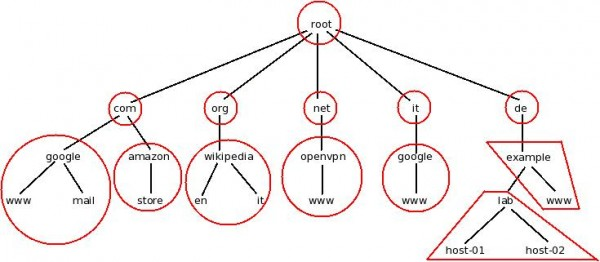
\includegraphics[scale=0.6]{dns.png}
\end{center}
I DNS, oltre alla risoluzione da nomi a IP, provvedono anche alla risoluzione inversa. Quest'ultima avviene tramite la gerarchia di zone \texttt{in.addr.arpa} (\texttt{ip6.arpa} per IPv6).\\
Le zone contengono diversi tipi di informazioni, memorizzate in record, tra cui
ricordiamo:
\begin{itemize}
\item SOA, che fornisce le informazioni generali sulla zona, tra cui un identificativo sequenziale della versione
della definizione (serial number), l'indirizzo email del responsabile e il tempo di vita (TTL) della definizione
della zona.
\item NS, che definisce quali siano i DNS responsabili per le richieste iterative riguardanti la zona.
\item MX, che definisce quali siano gli hostname dei server di posta in entrata responsabili per il dominio.
\item A, che rappresenta traduzioni nella forma da nome a ip. Per IPV6 il tipo corrispondente è AAAA.
\item CNAME, che rappresenta dei nomi alternativi (alias) per un host, nella forma da alias a nome.
\item TXT, che permette di associare stringhe arbitrarie ad un nome, nella forma da nome a stringa.
\item SRV, che permette di associare delle informazioni strutturate al nome di un servizio, nella forma da nomeservizio.protocollo a priorità peso porta nome host.
\item Il tipo PTR che, nelle zone per la risoluzione inversa, rappresenta le traduzioni nella forma da ip a nome.
\end{itemize}
I DNS possono essere gestiti in due modi:
\begin{itemize}
\item Tramite l'elenco contenuto nel file \texttt{/etc/hosts}
\item Tramite l'uso di un server DNS, in Linux è \textbf{BIND}
\end{itemize}
Alcuni comandi utili per la gestione dei DNS sono \texttt{host} e \texttt{dig}.\\
In Windows, oltre al sistema DNS, troviamo anche:
\begin{itemize}
\item WINS (Windows Internet Naming Service)
\item NetBEUI ( NetBIOS extended User Interface)
\item NetBIOS (Network Basic Input Output System): avete presente
quando nella rete di casa vostra sul file explorer scrivete
\texttt{\textbackslash \textbackslash pc\textbackslash cartella}? Quello
\end{itemize}
Tra i comandi utili, ricordiamo \texttt{netsh} e \texttt{nslookup}.\\
Nella stessa zona posso esserci più server dns,
di solito riconosciuti come master (primario)
contiene la copia principale del dabase dns e
propaga agli altri le modfiche, slave (secondario)
che possiede una replica, e caching.\\
Su Linux BIND, i files di configurazione li trovate in \texttt{/etc/bind}.\\

\chapter{Autenticazione}

\paragraph{Definizione.} Si intende una serie di problemi e operazioni
diverse che vanno dall'identificazione e
autenticazione (chi sei) alle autorizzazioni
vere e proprie (cosa vuoi e cosa puoi fare).\\
Storicamente, i sistemi UNIX usavano il contenuto \texttt{/etc/passwd}
per entrambi gli scopi. Il file contiene tante righe quanti sono gli
utenti del sistema, ed ognuna di queste ha la forma:\\
\tab \texttt{username:encpassword:UID:GID:gecos:homedirectory:shell}\\
\tab \texttt{gsportel:xZELC6ObSje96:1959:1000:Giorgia
Sportelli,,,:\\\tab/home/gsportel:/bin/sh}\\
Poiché alcune delle informazioni contenute nel file (ad esempio la
corrispondenza da username a UID) devono essere disponibili a tutti
gli utenti di sistema (ed in particolare alle loro applicazioni), il file
era (ed è) pubblicamente accessibile in lettura. La password era
protetta dalla (supposta) robustezza dell'algoritmo di hashing
usato, originariamente basato sull'algoritmo crittografico DES.\\
l file \texttt{/etc/group} contiene la lista dei gruppi del sistema e dei
relativi GID, nonché, per ognuno di essi, l'elenco dei suoi membri,
ad esclusione di quelli che hanno il suo GID come loro gruppo
primario. La sintassi di ogni riga del file:\\
\tab \texttt{groupname:encpassword:GID:listamembri}\\
Gli UNIX moderni non usano più direttamente il file
\texttt{/etc/passwd} per la funzionalità che gli da il nome, cioè la
memorizzazione della password. Questo ruolo è stato assunto dal
file \texttt{/etc/shadow}, che, servendo solo per la fase di
autenticazione, non è pubblicamente leggibile.\\
\tab \texttt{username:encpassword:ultimocambio:etàminima:etàmassima:\\\tab periodoavviso:periodoinattività:datascadenza:altro}\\
\paragraph{NSS e PAM.} Originariamente, tutti i file sopra indicati erano gestiti
direttamente dai programmi che ne richiedevano la
consultazione o la manipolazione (esempio vipw).\\
Ad ogni modifica dello standard del file era necessario
modificare anche i programmi che gestivano gli stessi.\\
Allo stesso modo, sistemi che storicamente
permettevano di centralizzare la gestione degli utenti
su più sistemi, come NIS, richiedevano una nuova
versione delle stesse utility.\\
Per ovviare a questa situazione, nel tempo sono nati
sistemi che permettono, tramite l'uso di componenti
modulari, di aggiungere meccanismi di autenticazione e
di gestione delle informazioni sugli utenti diversi, senza
per questo dover modificare i programmi che ne fanno
uso. In particolare, generalmente si usano:\\
\begin{itemize}
\item nss (Name Service Switch) per le informazioni sugli utenti,
nonché per altre mappe che associano nomi ad altre
informazioni.
\item PAM (Pluggable Authentication Modules) per i sistemi di
autenticazione.
\end{itemize}
Il sistema nss, in Linux, è parte dell'implementazione delle librerie C
del progetto GNU. Lo scopo del sistema è quello di fornire i dati dei
system database (tra cui \texttt{passwd} e \texttt{group}) alle applicazioni. Le
sorgenti dei dati, oltre ai file omonimi, possono essere le più disparate
(ad esempio mysql, ldap, ecc).\\
Dei moduli, anche di terze parti, si occupano di tradurre richieste e
risposte a/da questi database affinché possano essere effettuate sulla
fonte prescelta, come ad esempio una directory LDAP o un database
SQL. La configurazione di nss avviene principalmente tramite il file
\texttt{/etc/nsswitch.conf}, mentre moduli aggiuntivi si trovano,
solitamente, nei pacchetti Debian/Ubuntu dal nome \texttt{libnss-*}.\\
\texttt{nscd} è un daemon della cache di rete, ed è fondamentale per le performance in caso di autenticazione via rete.\\
Il sistema PAM fornisce i servizi d'autenticazione ad una o più
applicazioni/servizi (services), che possono avere configurazioni
separate. Le attività (task) di autenticazione stessa sono, in realtà,
suddivise in 4 management group:
\begin{itemize}
\item \textbf{account:} si occupa di verificare eventuali requisiti che l'account deve
rispettare, ad es. se è scaduto o se ha il permesso o divieto di accedere.
\item \textbf{auth(entication):} si occupa di autenticare l'utente e di acquisire le credenziali
necessarie.
\item \textbf{password:} si occupa di aggiornare/modificare le informazioni di
autenticazione. Un classico esempio è proprio l'operazione di cambio
password.
\item \textbf{session:} si occupa di gestire le attività che devono essere effettuate in
apertura ed in chiusura di una sessione, ad esempio
\begin{itemize}
\item all'accesso aggiorna I file \texttt{utmp} e \texttt{wmtp}, fa partire una sessione \texttt{sshagent}...
item all'uscita aggiorna I file \texttt{utmp} e \texttt{wmtp} termina la sessione \texttt{sshagent}...
\end{itemize}
\end{itemize}
Per ogni servizio ed ognuna di queste attività si possono
specificare una sequenza di operazioni tramite l'uso di moduli
(o plugin) intercambiabili.\\
Vi sono molti plugin di terze parti, che in Debian/Ubuntu sono
forniti in pacchetti dal nome \texttt{libpam-*}.\\
La configurazione si trova nei file nella directory
\texttt{/etc/pam.d/}, oppure, anche se sconsigliato, nel file
\texttt{/etc/pam.conf}.\\
I file in \texttt{/etc/pam.d/common-*}
indicano configurazioni
di default, che devono essere importate nei file che specificano
eventuali modifiche del comportamento standard.\\
\paragraph{La strada verso LDAP e KERBEROS, Active Directory e Autenticazione Centralizzata.}
In principio esisteva NIS, che sta per Network Information Services, fu sviluppato da Sun Microsystems
per centralizzare l'amministrazione di sistemi UNIX (in origine SunOS). Ora in
sostanza è diventato uno standard di settore; tutti i sistemi UNIX like (Solaris,
HP-UX, AIX, Linux, NetBSD, OpenBSD, FreeBSD, etc) supportano NIS.\\
NIS in precedenza era noto come Yellow Pages, ma per una questione di marchi,
Sun ha cambiato il nome. Il vecchio termine (e yp) è ancora si incontra ancora
spesso.\\
E' un sistema client/server basato su RPC che permette ad un gruppo di macchine
in un dominio NIS di condividere un insieme comune di file di configurazione.
Questo permette ad un amministratore di sistema di installare sistemi client NIS con
il minimo di dati di configurazione e di aggiungere, rimuovere o modificare dati di
configurazione da una singola macchina.\\
Questo sistema era molto insicuro, in quanto tutto viaggiava in chiaro. Bastava diventare root di un client per accedere a tutte le informazioni del database NIS.\\
Poi arrivò NIS+, con una struttura gerarchica con server principali e di backup, e autenticazione tramite password criptata. Ora non è più supportato.\\
Tornando ai giorni nostri: LDAP (Lightweight Directory Access
Protocol) è un protocollo per l'interrogazione e
la manipolazione di directory, ovvero basi di
dati che seguono un modello gerarchico.\\
Viene utilizzato in ambiti in cui, il numero delle
operazioni di consultazione (lettura) può
essere elevato, mentre le operazioni di
modifica (scrittura) sono relativamente rare.\\
DIT (Directory Information Tree): è l’albero dei dati contenuti in un database
ldap.\\
I nodi rappresentano suddivisioni di vario tipo (ad esempio gli uffici di una
organizzazione). Le foglie sono i dati veri e propri.\\
Ogni nodo (entry) dell'albero ha un relative distinguished name (RDN), che è
unico tra tutti i nodi fratelli. Mentre la sequenza di tutti gli RDN dalla radice fino al
nodo interessato viene chiamato Distinguished Name (DN), ed è unico per
tutto il DIT.\\
I nodi possono avere informazioni strutturate (ad esempio nome, cognome,
email, numero di telefono...) organizzate in attributi, ed implementare uno o
più schemi (ing. schema), che non sono altro che delle definizioni di tipi di dato.\\
I nodi possono anche indicare dei riferimenti ad altre parti del DIT, o addirittura a
DIT di altri server LDAP (referral).\\
\begin{center}
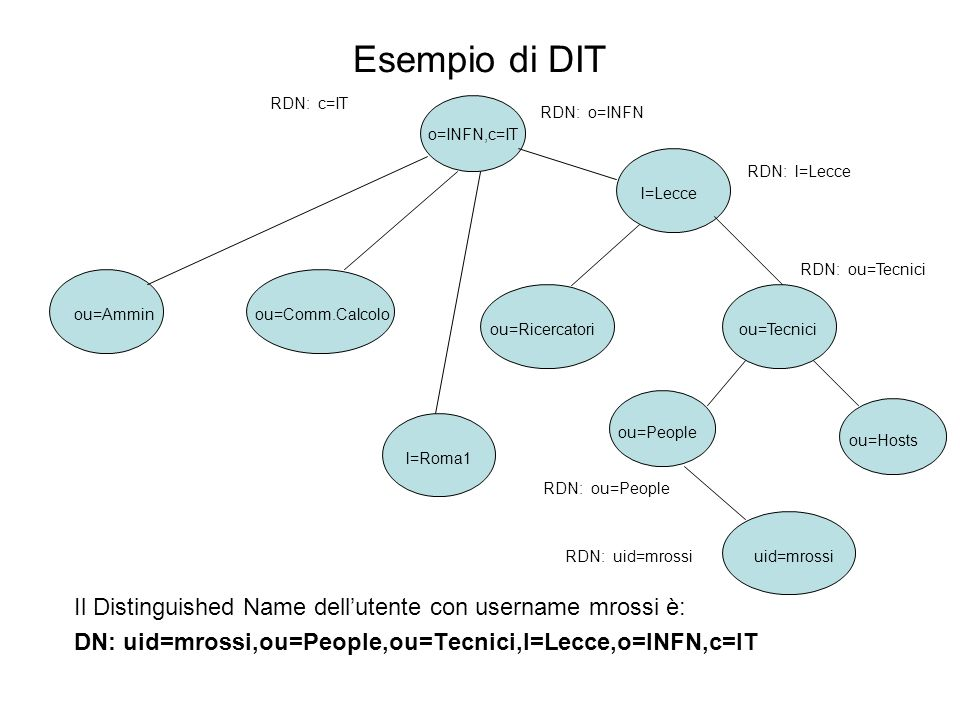
\includegraphics[scale=0.5]{dit.png}
\end{center}
L'accesso alla directory ldap può essere
anonimo oppure tramite autenticazione
(binding). La fonte dei dati d'autenticazione può
essere interna al DIT o esterna.\\
Vi sono molte implementazioni di server LDAP.
Le più note nei sistemi UNIX sono OpenLDAP
(pacchetto Debian/Ubuntu slapd) e 389 Directory
Server.\\
Su Windows si utilizza Active Directory (con Kerberos).\\

LDAP è spesso usato per fornire le informazioni sugli utenti
e sui gruppi ad un insieme di elaboratori. Il sistema nss
dispone di un plugin (pacchetto Debian/Ubuntu \texttt{libnss-ldap})
che, attivato e configurato opportunamente,
consente di usare dei server ldap come fonte per i vari
database di sistema.\\
LDAP, qualche volta, è anche usato (tramite \texttt{libpam-ldap})
per l'autenticazione, facendo verificare al sistema
locale se la password cifrata presente nel DIT (esattamente
come in \texttt{/etc/passwd} o \texttt{/etc/shadow}) corrisponde a
quella immessa dall'utente, oppure cercando di autenticarsi
(binding) al server LDAP stesso usando quelle credenziali.\\
Kerberos è un sistema per l'autenticazione
distribuita basato sulla crittografia. Il
protocollo si affida ad un insieme limitato di
nodi fidati che fanno da arbitro alla situazione
richiedendo e fornendo prove dell'avvenuta
identificazione ed autenticazione delle parti.\\
I sistemi che usano una stessa infrastruttura
basata su Kerberos formano un Realm, che ha
un nome ben definito.\\
\paragraph{Schema di funzionamento di Kerberos:}
\begin{itemize}
\item AS\_REQ è la richiesta iniziale di autenticazione dell'utente (fatta con il kinit tanto per
intenderci). Tale messaggio è diretto alla componente del KDC nota come Authentication Server
(AS);
\item AS\_REP è la risposta dell'Authentication Server alla richiesta precedente. Sostanzialmente
contiene il TGT (criptato con la chiave segreta del TGS) e la chiave di sessione (criptata con la
chiave segreta dell'utente richiedente);
\item TGS\_REQ è la richiesta da parte del client rivolta al Ticket Granting Server (TGS) per un ticket
di servizio. Dentro questo pacchetto viaggia il TGT ottenuto dal messaggio precedente e un
autenticatore generato dal client e criptato con la session key;
\item TGS\_REP è la risposta del Ticket Granting Server alla richiesta precedente. Ci si trova dentro
il service ticket richiesto (criptato con la chiave segreta del servizio) e una chiave di sessione di
servizio generata dal TGS e criptata con la precedente chiave di sessione generata dall'AS;
\item AP\_REQ è la richiesta che il client manda ad un server applicativo per accedere ad un servizio.
Le componenti sono il ticket di servizio ottenuto dal TGS con la risposta precedente e un
autenticatore generato sempre dal client, ma questa volta criptato con la chiave di sessione del
servizio (generata dal TGS);
\item AP\_REP è la risposta che il server applicativo dà al client per provare di essere veramente il
server che il client si aspetta. Questo pacchetto non è sempre richiesto. Il client lo richiede al
server solo quando è necessaria la mutua autenticazione.
\end{itemize}
\begin{center}
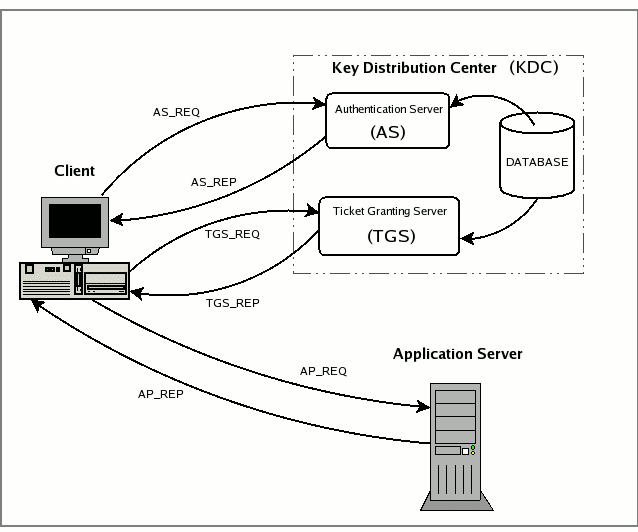
\includegraphics[scale=0.5]{kerberos.png}
\end{center}
Esistono diverse implementazioni di Kerberos. In ambiente UNIX le più note
sono MIT Kerberos e Heimdal. Mentre il protocollo Kerberos è standard, e
pertanto le implementazioni sono interoperabili, alcune funzionalità di
amministrazione, che usano un protocollo ad hoc, possono non esserlo.
\\Tramite il modulo PAM appropriato (pacchetto \texttt{libpam-krb5})
è possibile
far autenticare un utente del sistema usando le sue credenziali Kerberos. Il
modulo si occuperà anche di far avere un TGT all'utente, che così potrà
usare altri servizi che partecipano al realm senza dover fornire nuovamente
la password.
\\Sebbene anche i servizi possano usare Kerberos attraverso PAM, questo
non permette la funzionalità di single sign-on appena descritta, né altre
caratteristiche avanzate di Kerberos. Pertanto i servizi che lo richiedono
spesso usano Kerberos per conto loro o attraverso GSSAPI (Generic
Security Service Application Program Interface).\\
Active Directory è un database ldap integrato nei server Windows
($\geq$ 2000), che fungono da Domain Controller, e consente di catalogare e
gestire in modo centralizzato risorse di vario genere come: utenti, gruppi di
lavoro, stampanti, cartelle condivise, ecc.
\\La struttura del database è di tipo gerarchico, con contenitori che
contengono oggetti e altri contenitori.
\\Sostanzialmente è una implementazione limitata di ldap + kerberos.
\\Il primo procedimento da attuare e definire la struttura di Active Directory.
Active Directory è un contenitore di oggetti, ovvero utenti, gruppi, computer,
server, stampanti, unità organizzative.
\\Per la realizzazione di un dominio active directory è sufficiente lanciare il
comando \texttt{dcpromo.exe}. Il sistema si occuperà da solo di creare tutto ciò
che serve per l'autenticazione centralizzata, tra cui anche un server DNS.\\
Importanti per un corretto funzionamento di
ldap, kerberos e active directory sono:
\begin{itemize}
\item Sincronizzazione degli orologi (NTP).
\item Corretta configurazione dei DNS sia diretta che
inversa.
\item Correttezza dei certificati SSL.
\item Manutenzione costante del database utenti/gruppi.
\end{itemize}
\chapter{Posta}
La posta è uno dei servizi più diffusi e importanti della rete Internet.
\paragraph{Struttura } Il servizio di posta è così strutturato:
\begin{itemize}
\item \textbf{Mail User Agent:} client di posta, ovvero un programma usato da un utente per inviare/visualizzare messaggi, può anche essere una webapp.
\item \textbf{Mail Submission Agent:} si occupa di ricevere i messaggi da un MUA e inviarli ad un MTA.
\item \textbf{Mail Transit Agent:} si occupa di ricevere mail da un MSA o da un altro MTA, e a instradarle a un altro MTA oppure a un LDA.
\item \textbf{Mail Delivery Agent o Local Delivery Agent:} si occupa di consegnare il messaggio alla casella di posta dell'utente indicato qualora la destinazione finale del messaggio sia nel sistema corrente.
\item \textbf{Mail Access Agent:} permett di visualizzare/scaricare i messaggi.
\item \textbf{Mail Retrival Agent:} scarica la posta da un MAA e la rende disponibile in locale.
\end{itemize}
Va tenuto conto che MSA è integrato nel MTA, e MRA è integrato nel MUA.\\
Il servizio di Posta segue un certo flusso:
\begin{enumerate}
\item Un utente (mittente) scrive una email usando un MUA.
\item MUA invia la mail ad un MSA/MTA.
\item MTA controlla l'indirizzo di destinazione (\texttt{utente@dominio}):
	\begin{itemize}
	\item Se il dominio è tra quelli serviti da MTA in questione (indirizzo locale) e utente è effettivamente valido, questa viene girata al LDA, che la consegna nella casella di posta associata, e il viaggio termina; altrimenti, MTA rifiuta il messaggio.
	\item Se invece l'indirizzo non è locale, MTA accetta di instradare il messaggio (relay), mette il messaggio in una coda d'uscita e procede.
	\end{itemize}
\item Dopo aver estratto dalla coda il messaggio, il MTA controlla quale sia il record MX associato al dominio o, se non presente, un record 'A' (relativo al nome DNS dell'host dato), e contatta l'MTA che risponde a quell'host, cercando di inviargli il messaggio.
	\begin{itemize}
	\item Se l'invio avviene correttamente, il messaggio è gestito da MTA di destinazione, che procede dal punto \texttt{2)}.
	\item Se MTA contattato non risponde, il messaggio torna in coda.
	\item Se MTA contattato rifiuta il messaggio, oppure se il messaggio è stato troppo tempo in coda, viene mandata una mail all'indirizzo indicato dal mittente, notificando la mancata consegna, e il procedimento termina.
	\end{itemize}
\item A questo punto il messaggio si trova nella \texttt{inbox} del destinatario.
\end{enumerate}
\begin{center}
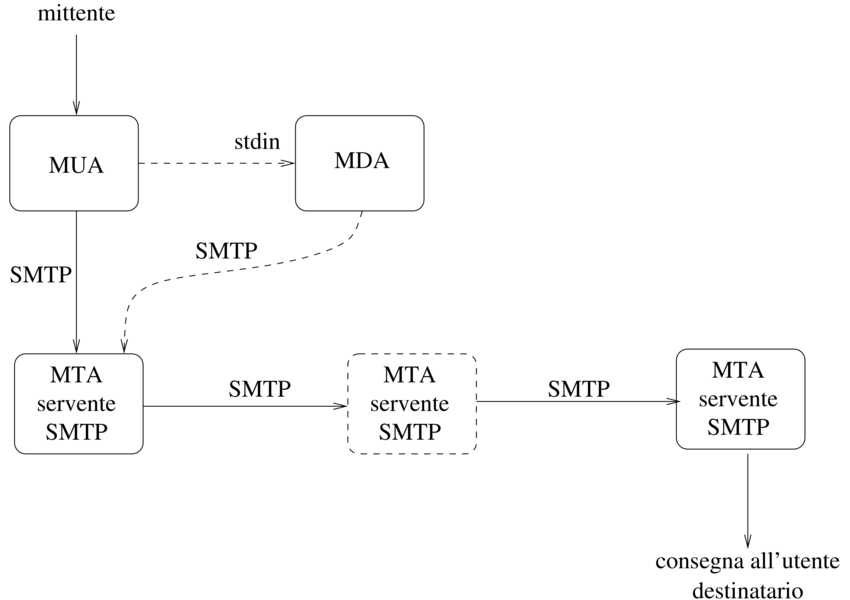
\includegraphics[scale=0.5]{flussoposta.png}
\end{center}
Il flusso, così com'è, non garantisce in alcun modo la consegna, la notifica degli errori, l'identità del mittente o la privatezza della comunicazione.\\
Per ovviare a questi problemi, bisogna ricorrere a sistemi a livello applicazione.\\
Il relay non è sempre concesso. Si accetta in due casi:
\begin{itemize}
\item Se la richiesta viene da un host conosciuto (es.: la propria rete aziendale).
\item Se l'utente è autenticato.
\end{itemize}
In tutti gli altri casi il messaggio viene rifiutato immediatamente.\\
\paragraph{Protocolli} Il protocollo usato tra MUA e MTA e tra MTA e MTA si chiama \textbf{SMTP} (Simple Mail Transfer Protocol) o ESMTP (Extended SMTP). La comunicazione tra MTA e LDA può avvenire sia internamente (es.: tramite scambio di file e/o memoria condivisa tra le componenti), oppure tramite \textbf{LMPT} (Local Mail Transfer Protocol), che è una versione semplificata di ESMTP. La connessione tra MAA e MUA avviene tipicamente tramite \textbf{POP3} (Post Office Protocol versione 3) o \textbf{IMAP4} (Internet Message Access Protocol versione 4). \\
\paragraph{Differenze tra POP e IMAP:}
\begin{itemize}
\item \textbf{IMAP} conserva le mail sul server; la lettura, l'invio e la gestione possono avvenire anche da client desktop, ma è il server a mantenere la copia delle mail inviate, ricevute e scritte; quindi con IMAP le mail sono disponibili da qualsiasi dispositivo.
\item \textbf{POP} invece delega al dispositivo usato per la consultazione il compito di provvedere al salvataggio; le mail vengono scaricate sul dispositivo e la connessione è necessaria solo per inviare e ricevere posta; in realtà, i MUA hanno delle opzioni per POP che permettono di mantenere una copia dei messaggi sul server.
\end{itemize}
\textbf{Sendmail } fu il primo MTA a fare uso di SMTP. Venne utilizzato fino al 2005 come MTA da moltissimi server di posta, ma purtroppo la progettazione rigida e la complessità della configurazione lo resero via via meno popolare, fino all'estinzione. Un altro aspetto da considerare, era la presenza di numerosi bug e problemi di sicurezza.\\
Altri MTA degni di nota sono:
\begin{itemize}
\item Qmail: ideato da Dan Bernstein circa 10 anni fa, è un server di posta
scalabile, performante, sicuro e portabile. Si dice sia il più sicuro...
Attualmente è il secondo MTA più usato su internet. (Per approfondire:
http://www.qmail-ldap.info).
\item Courier MTA: è un server di posta/groupware integrato che poggia su vari
protocolli: ESMTP, IMAP, POP3, SSL e HTTP. Sostanzialmente offre tutti i
servizi di posta elettronica compreso anche un sistema di webmail. È quindi
una soluzione completa per la gestione della posta, volendo è simile a
Exchange. (http:// www.courier-mta.org)
\item Exim: MTA standard di Debian fino a qualche versione fa.
\item Zimbra: suite completa per la gestione della posta (http://zimbra.org).
\item Postfix.
\item Exchange.
\end{itemize}
\begin{center}
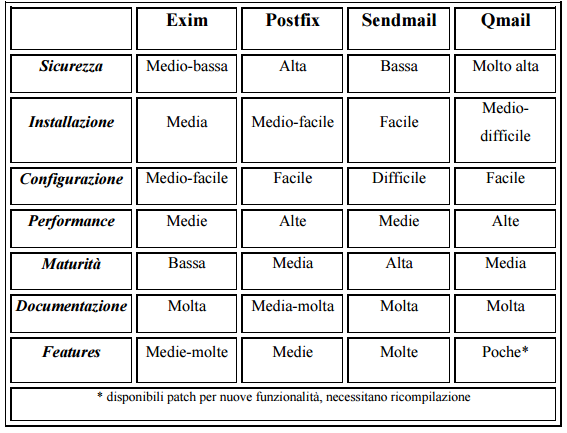
\includegraphics[scale=0.62]{confrontomta.png}
\end{center}
\textbf{Postfix} è il MTA di riferimento in ambiente Linux; è facile da configurare, è modulare, e permette di utilizzare diversi tipi di autenticazione. Permette inoltre di interfacciarsi facilmente con altri sistemi di controllo della posta:
\begin{itemize}
\item Real-time Blackhole List (RBL): viene bloccata una lista di indirizzi IP che sono ritenuti responsabili dell'invio di spam.
\item Sender Policy Framework (SPF): sistema di validazione mail progettato per riconoscere le mail provenienti da un indirizzo contraffatto (\texttt{spoofing}) che funziona grazie ad un meccanismo che permette al MTA di vedere se una mail arriva da un dominio autorizzato da chi amministra l'host.
\item Sistemi di greylisting: metodo per difendersi dallo spam che consiste nel rifiutare temporaneamente tutte le mail da un mittente sconosciuto, in quanto se la mail è legittima il mailserver del mittente ritenterà l'invio; questo discorso era valido finché gli spammer non hanno capito che bastava rinviare le mail per bypassare la greylist.
\item Sistemi antispam basati sul contenuto (i.e.: SpamAssassin): sistemi che filtrano le mail basandosi sul contenuto della mail.
\item Sistemi antivirus e molto altro (i.e.: ClamAV).
\end{itemize}

\textbf{MS Exchange} è un software studiato per agevolare la collaborazione in linea tra vari utenti. Venne introdotto nel 1996 da Microsoft e oggi è uno dei mailserver più potenti e utilizzati. Tra le sue funzionalità più rilevanti, la gestione centralizzata della posta elettronica, dei calendari e delle rubriche contatti, che possono essere condivisi tra i vari utenti di una rete aziendale. Il client più utilizzato per connettersi a un server Exchange è MS Outlook, disponibile nella suite Office. È disponibile anche una webapp (Outlook Web Access) per l'accesso da browser.\\

\textbf{MAA Dovecot} permette di usare i protocolli IMAP e POP3 e supporta, sia in consultazione che in consegna, diversi formati di memorizzazione della posta, quali \texttt{mbox, maildir, dbox}. Permette inoltre, tramite un plugin, di avere un sistema di filtri server side con cui smistare la posta degli utenti in vari folder, nonché poterla inoltrare ad altri indirizzi. Per gestire questi filtri lato server si usa il protocollo SIEVE. Consente anche di gestire la quota della posta per ogni utente, di adottare vari metodi di autenticazione tramite SQL, LDAP, ecc..\\

\paragraph{Spam:} uno o più messaggi non richiesti, inviati o postati come parte di un più grande insieme di messaggi, tutti con il medesimo contenuto.\\
Possiamo dividere lo spam in cinque categorie:
\begin{itemize}
\item \textbf{Hoax:} bufale o catene di messaggi.
\item \textbf{Worm:} mail mandate da un virus.
\item \textbf{UCE:} Unsoliticed Commercial Email, ovvero mail di carattere commerciale non richieste.
\item \textbf{UBE:} Unsoliticed Bulk Email, ovvero mail indesiderate mandate in grande quantità.
\item Messaggi derivanti da mailing list.
\end{itemize}

Le maggiori fonti di spam sono UCE e UBE. La prevenzione e la lotta allo spam non sempre sono facili, in quanto vengono sempre creati nuovi metodi per far pervenire le mail indesiderate alle nostre caselle di posta.\\
Appare evidente che il problema dello spam non è arginabile da una policy statica, per quanto possa essere complessa. Possiamo solo decidere di filtrare le mail in ingresso con vari meccanismi di filtraggio, ma tenendo conto che non deve essere totale in quanto si rischierebbe di compromettere il servizio mail scartando delle mail legittime.\\
\paragraph{Greylisting:} tecnica di difesa dallo spam che consiste nel rifiutare la mail proveniente da un dominio sconosciuto per un numero \texttt{N} di volte. Ad ogni rifiuto, MTA sender rimette la mail in coda e dopo un certo periodo di tempo \texttt{T} ritenta l'invio. Al tentativo \texttt{N}, la mail viene accettata e MTA di invio viene inserito in una whitelist, in modo da considerare legittime le mail provenienti da questo.\\
Il greylisting è una tecnica che sta perdendo efficacia, in quanto i programmi che si occupano dell'invio dello spam sono ingrado di reinviare più volte la mail, aggirando il sistema; inoltre, possono verificarsi ritardi nella consegna delle mail. L'aspetto positivo è che con questo sistema, nessuna mail lecita viene scartata.\\
In postfix, il greylisting è implementato grazie ai demoni \texttt{postgrey} o \texttt{policyd}.
\paragraph{RBL:} sono "liste nere" contenenti un elenco di indirizzi IP che non sono autorizzati ad inviare email.\\
Non è facile distinguere gli indirizzi IP validi da quelli di spam, e spesso vengono scartate delle mail lecite. Spesso quindi vengono implementati dei criteri di utilizzo "personali", e vengono gestite da terze parti.\\
Alcuni criteri per la selezione degli IP da bloccare includono il blocco di tutti gli IP assegnati dinamicamente dal provider, il blocco di tutti gli IP che inviano mail senza passare da un mail server ufficiale e il blocco di IP segnalati come spammer dagli utenti.\\
In postfix si attiva RBL alla direttiva \texttt{reject\_rbl\_client} alla voce \texttt{smtpd\_recipient\_restrictions}:\\
\tab\texttt{reject\_rbl\_client zen.spamhaus.org}
\paragraph{SPF:} non si tratta di una vera e propria tecnica di difesa dallo spam, ma piuttosto di uno standard che si applica in ambito di risoluzione dei DNS per cui si può dichiarare, tramite un record di testo, quali sono gli indirizzi IP o nomi che possono inviare mail per il dominio stesso.\\
Si crea sostanzialmente una maschera per cui il mailserver ricevente, se il record ha la giusta formattazione, può verificare se il server mittente è abilitato a inviare.\\
Questo comporta non poche problematiche:
\begin{itemize}
\item Sono ancora molti i domini che non implementano il suddetto record.
\item L'implementazione può essere difficoltosa sulle strutture mail di una certa complessità.
\item Si complica il processo di forwarding (inoltro) delle mail.
\end{itemize}
In postfix ci si rifà alla direttiva \texttt{smtpd\_recipient\_restrictions}, inserendo la voce:\\
\tab\texttt{check\_policy\_service spf}
\paragraph{Spamassasin:} è una tecnica di difesa dallo spam che utilizza un sistema di filtri euristici, ovvero il sistema prova a "indovinare" se la mail è valida o meno assegnandole un punteggio sulla base di vari aspetti, come per esempio la lingua della mail, la presenza di tag \texttt{html} o la presenza di parole chiave.\\
A seconda del punteggio ottenuto dalla mail, spamassasin può decidere di lasciar passare la mail, applicare dei tag all'oggetto della mail per segnalarla all'utente come spam, oppure scartarla.\\
Il vantaggio è che può essere "istruito" in base alle mail ricevute in precedenza, e di conseguenza migliorare la sua efficacia se si verificano determinate condizioni nelle mail ricevute in precedenza.\\
Per essere correttamente configurato necessita di continui aggiustamenti fatte da personale con una certa esperienza.\\
In postfix si presenta con il daemon \texttt{spamassassin}.
\paragraph{Controlli MTA:} MTA può implementare dei controlli per ridurre il flusso dello spam automatizzato.\\
Ad esempio, in postfix:
\begin{itemize}
\item \texttt{smtpd\_helo\_required = yes} controlla che il sender inizi la comunicazione con il comando \texttt{ehlo}.
\item \texttt{smtpd\_helo\_restrictions} controlla chi può iniziare un dialogo tramite il comando \texttt{ehlo}. I parametri sono:
	\begin{itemize}
	\item \texttt{permit\_sasl\_authenticated}
	\item \texttt{permit\_mynetworks}
	\item \texttt{reject\_non\_fqdn\_hostname}
	\item \texttt{permit}
	\item ...
	\end{itemize}
\item \texttt{smtpd\_sender\_restrictions} controlla chi possa inviare mail dopo essersi identificato con \texttt{ehlo}. I parametri sono:
	\begin{itemize}
	\item \texttt{permit\_sasl\_authenticated}
	\item \texttt{permit\_mynetworks}
	\item \texttt{reject\_non\_fqdn\_sender}
	\item \texttt{permit}
	\item ...
	\end{itemize} 
\item \texttt{smtpd\_recipient\_restrictions} effettua controlli sul destinatario. I parametri sono:
	\begin{itemize}
	\item \texttt{check\_policy\_service}
	\item \texttt{inet:127.0.0.1:10031}
	\item \texttt{reject\_non\_fqdn\_recipient}
	\item \texttt{permit}
	\item ...
	\end{itemize} 
\end{itemize}

\paragraph{AMAVIS:} è un sistema che filtra i contenuti delle mail, implementando il trasferimento, l'elaborazione e la codifica delle stesse, interfacciandosi con altri sistemi di filtraggio di spam e virus.\\
Può essere visto come un'interfaccia tra un MTA e altri sistemi di filtraggio, come spamassassin.\\
Può essere usato per rilevare virus, spam, contenuti vietati nella mail, etichettatura, blocco e spostamento delle mail a seconda del loro contenuto, messa in quarantena o rilascio dei messaggi, eliminazione dei virus dai messaggi grazie ad antivirus esterni, ecc..\\
Una configurazione comune di Amavis è quello di avere un sistema di filtraggio basato su:
\begin{itemize}
\item Postfix
\item Spamassassin
\item ClamAV
\item Amavis
\end{itemize}
In postfix è presente come daemon \texttt{amavisd-new}.
\begin{center}
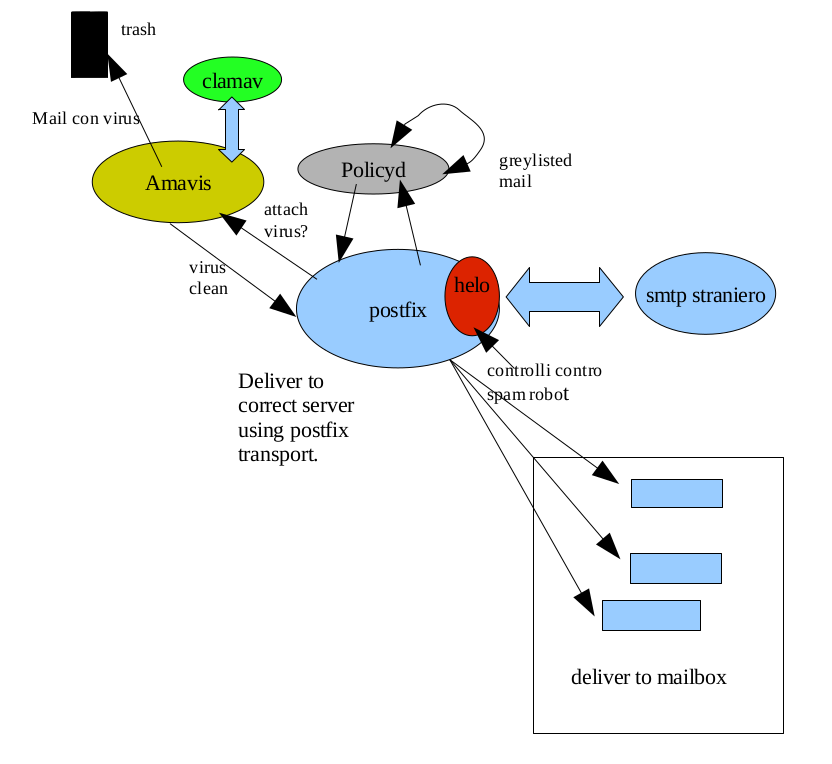
\includegraphics[scale=0.5]{esempioamavis.png}\\
\end{center}

Per installare postfix si utilizza il comando:\\
\tab\texttt{\#apt-get install postfix}\\
I files di configurazione sono presenti in \texttt{/etc/postfix}.\\
per installare dovecot si utilizza il comando:\\
\tab\texttt{\#apt-get install dovecot dovecot-imapd dovecot-pop3d dovecot-lmtpd}\\
I files di configurazione in \texttt{/etc/dovecot}.\\
\begin{center}
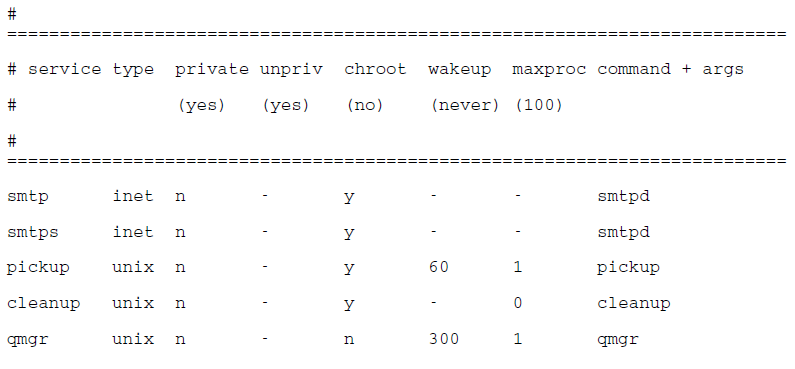
\includegraphics[scale=0.5]{post1.png}\\
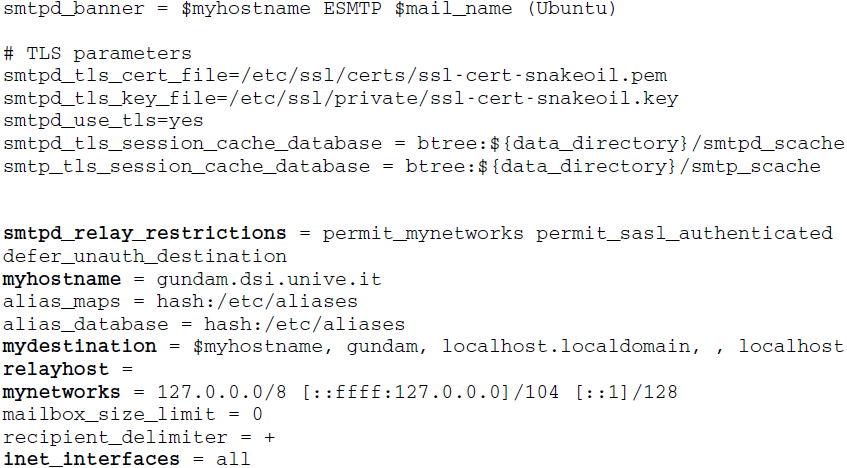
\includegraphics[scale=0.5]{post2.png}\\
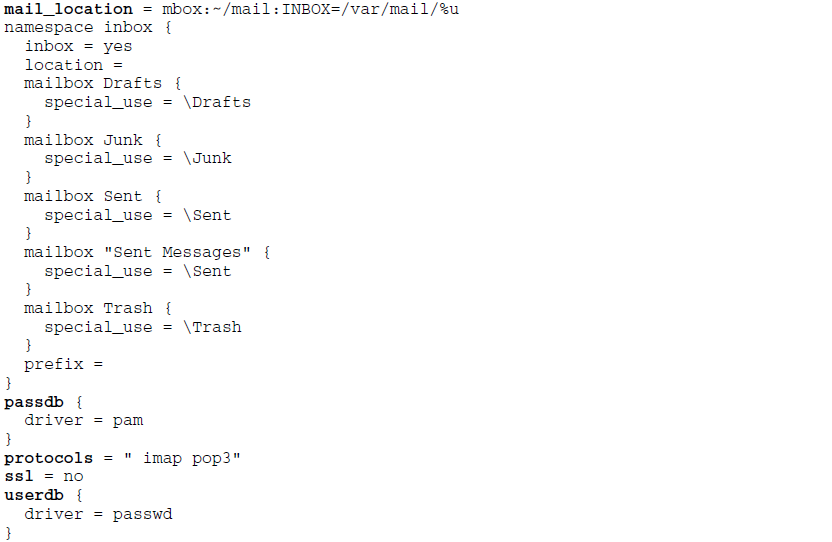
\includegraphics[scale=0.5]{post3.png}
\end{center}

\chapter{Filesystem Distribuito}
Il filesystem distribuito è un particolare tipo di filesystem che permette la memorizzazione dei files e delle risorse in dispositivi di archiviazione distribuiti in una rete informatica.\\I dati non sono archiviati su un dispositivo locale ma, attraverso un sistema client/server, su dispositivi remoti collegati in modo trasparente alla propria gerarchia dei file.\\Un DFS deve gestire i files in modo concorrente e trasparente, e può essere dotato di autenticazione e criptazione.\\
\paragraph{File Server:} è un server che ospita un DFS offrendo una serie di servizi ai client che lo sfruttano. Sui client è installata un'interfaccia al file server che include delle operazioni che normalmente si fanno sui files locali.\\
Su NFS e CIFS questa interfaccia è trasparente: si utilizzano i comandi di sistema sui files come se fossero locali.\\
Il file server controlla un insieme di dispositivi di memoria di massa su cui agisce in base alle richieste dei client.\\
Un file server, per regola generale, deve essere replicato e ridondato.\\
In un filesystem distribuito i dispositivi di memorizzazione sono dislocati in una rete. Le richieste e le risposte devono, pertanto, essere trasportate attraverso tale rete. La differenza principale sta nel fatto che invece di avere un dispositivo unico e centralizzato, il sistema ne può avere molti e indipendenti.\\
Le implementazioni di un filesystem distribuito possono variare:
\begin{itemize}
\item In alcune occasioni il server (file server) viene eseguito su una macchina dedicata.
\item Il sistema client può accedere simultaneamente a più file servers.
\item La stessa macchina può ospitare sia un server che un client.

\end{itemize}
Idealmente un FS distribuito appare all'utente come un normale FS centralizzato, in quanto molteplicità e dispersione di server e dispositivi a cui si riferisce possono essere celati. L'interfaccia rivolta alle applicazioni che usa l'utente non dovrebbe poter distinguere i file locali da quelli remoti, in quanto è compito del FS distribuito trovare e trasportare i dati attraverso la rete. L'aspetto che incide maggiormente sul lato utente sono le prestazioni del FS distribuito.\\
Per valutare le prestazioni di un FS distribuito si quantifica l'ammontare di tempo impiegato per soddisfare una data richiesta. Nei sistemi convenzionali questo consiste nell'accesso al disco locale e ad una piccola quantità di elaborazione da parte della CPU. Nei sistemi distribuiti, invece, si somma il ritardo dovuto alle comunicazioni di rete: questo ritardo include il tempo necessario a sottoporre la richiesta al server e quello per ottenere la risposta attraverso la rete, mentre occorre sommare il tempo necessario alla CPU per manipolare il protocollo di comunicazione in ciascuna direzione. Le prestazioni di un FS distribuito incidono sul suo livello di trasparenza, in quanto un sistema distribuito dovrebbe avere una velocità paragonabile a quella di un sistema convenzionale.\\
Un FS distribuito deve provvedere sia all'accesso dei client ai files, ma anche alla loro modifica: gli aggiornamenti operati da un client non possono però interferire con gli accessi e le modifiche fatte da altri client. Sono quindi necessari meccanismi di controllo della concorrenza e locking che possono essere inclusi nella realizzazione del FS distribuito, oppure resi disponibili da un protocollo parallelo.\\
Nel tempo sono stati sviluppati diversi DFS, in particolare:
\begin{itemize}
\item \textbf{NFS:} il primo DFS a essere sviluppato (dalla SUN nel 1985), diffuso e molto usato, ora è alla versione 4.
\item \textbf{AFS}
\item \textbf{CIFS/SMB}
\item \textbf{Google FS}
\item \textbf{Coda, Plan9, xFS}
\end{itemize}
\paragraph{NFS:} usa un remote access model, dove i nodi client non sanno realmente dove sono i files, e i server esportano una serie di operazioni sui files. \\
Altri sistemi usano un modello upload/download:
\begin{itemize}
\item Il nodo client scarica il file in una cash locale.
\item A modifiche avvenute, il file viene caricato sul server.
\item Il server dovrebbe mantenere le versioni dei files; tra i sistemi di versioning utilizzabili: SVN, GIT, CVS.
\end{itemize}
NFS è indipendente dall'organizzazione del FS locale, e per questo riesce a integrare i FS di Unix, Linux, Windows e OS X.\\
Esporta all'utente una visione simile a quella dei FS Unix-like basati su files organizzati come sequenze di bytes. Utilizza RPC come protocollo sottostante, ovvero un client fa una richiesta remota di esecuzione di una subroutine per la gestione dei files.\\
Dalla versione 4 supporta server non stateless (che richiedono, quindi, il ricevimento di un ACK seguente all'invio di un pacchetto). I client dovevano mantenere lo stato delle operazioni correnti su un FS remoto, ma nella versione 4 i server NFS mantengono lo stato delle operazioni. A partire dalla versione 4, inoltre, è stato introdotto il supporto del TCP, mentre prima era utilizzabile UDP.\\
Nella versione 4, NFS ha introdotto le compound procedure, che comprendono più richieste di operazioni in una singola chiamata, riducendo così il numero di chiamate RPC (offrendo, quindi, prestazioni migliori).\\
Riguardo le compound procedures, va tenuto conto che:
\begin{itemize}
\item Se un'operazione in una compound procedure fallisce, le successive operazioni non vengono eseguite.
\item Viene ritornato un messaggio con le informazioni sulle operazioni eseguite e l'errore che si è verificato.
\item Non conviene inviare operazioni non correlate tramite una compound procedure.
\end{itemize}
Quando si tratta di un FS wide area, è bene implementare file locking, protocolli di cache consistency e procedure ci callback.\\
Riassumendo:
\begin{itemize}
\item NFSv4 si basa sul protocollo TCP.
\item Il server deve mantenere delle informazioni di stato.
\item Il riconoscimento dell'utente avviene tramite una stringa arbitraria (es.: username); la traduzione di queste stringhe e le informazioni necessarie a cliente e server avviene tramite un \texttt{id mapper} (daemon \texttt{imapd}).
\item L'identità degli utenti può essere provata tramite sistemi di autenticazione esterni (Kerberos).
\item Vengono introdotte nel protocollo delle possibili migliorie delle prestazioni (es.: le deleghe) e per l'affidabilità (supporto per la replicazione, che però non è implementata direttamente nel protocollo).
\end{itemize}
Per installare NFS in ubuntu/debian:\\
\tab\texttt{\# apt-get install nfs-kernel-server} (sul server)\\
\tab\texttt{\# apt-get install nfs-common} (sul client)\\
Per la configurazione, editare \texttt{/etc/exports}, che ha la sintassi \texttt{/percorso cartellacondivisa indirizzoip (opzioni)}. Ecco alcuni esempi:\\
\tab\texttt{/home 157.138.22.21(rw, no\_root\_squash)}\\
\tab\texttt{/home 157.138.0.0/16
(rw,async,no\_subtree\_check,sec=krb5:krb5i:krb5p)}\\
Per la gestione del servizio, invece:\\
\tab\texttt{\# service nfs-kernel server restart}\\
\begin{center}
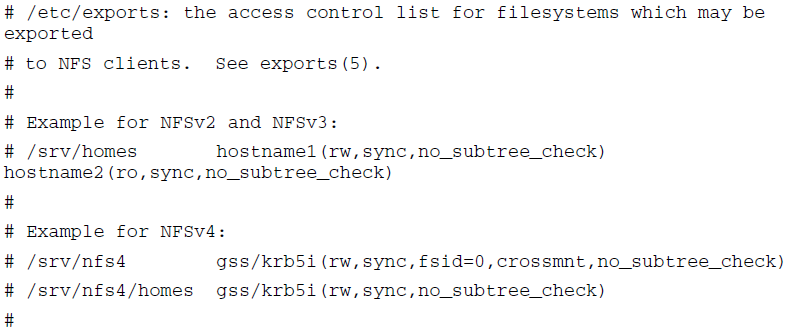
\includegraphics[scale=0.60]{fsesempioconf.png}
\end{center}
Per utilizzare l'area condivisa ho tre modi:
\begin{itemize}
\item Effettuando il mount manuale:\\
	\tab\texttt{\# sudo mount 192.168.1.1:/home /mnt/nfs/home}
\item Inserendo il mount \texttt{/etc/fstab} in modo che sia montato in avvio:\\
	\tab\texttt{192.168.1.1:/home /mnt/nfs/home nfs rw,user,auto 0 0}
\item Usando \textbf{automount}: soluzione migliore in caso di molti client e molti utenti che non hanno accesso diretto all'utente amministratore (\texttt{root}) e/o ai files di sistema (\texttt{/etc/fstab}).
\end{itemize}
\begin{center}
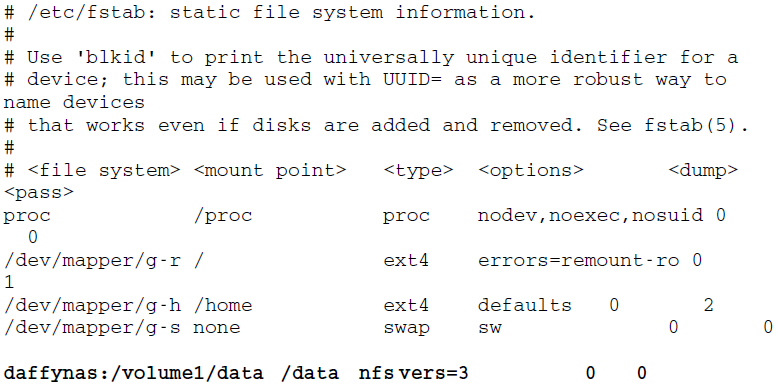
\includegraphics[scale=0.6]{esdfs1.png}\\
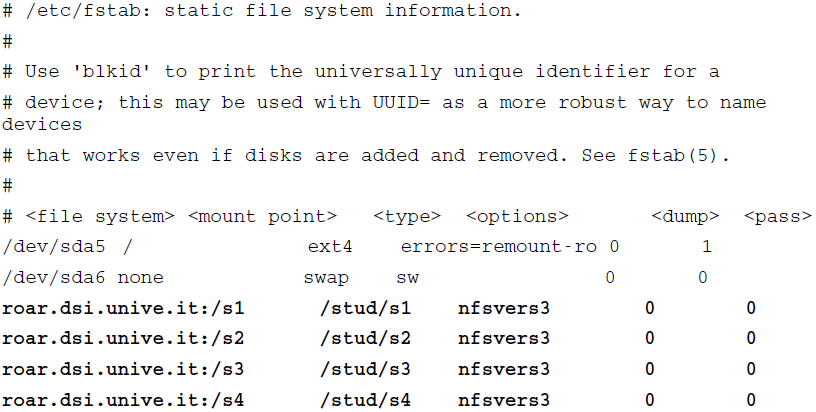
\includegraphics[scale=0.6]{esdfs2.png}
\end{center}
\paragraph{Automount} Non è mai consigliabile mantenere un FS remoto montato permanentemente su un sistema. In caso di fallimenti della rete, le operazioni che interessano dei files presenti nelle partizioni montate potrebbero essere bloccate. Inoltre, se si montano separatamente una gran quantità di posizioni (es.: le directories \texttt{home} degli utenti) in alcuni unix si rischia di eccedere il numero massimo di mount.\\
Per questo vari sistemi Unix (tra cui Linux) implementano un meccanismo di automount: quando un processo accede a un file o a una directory all'interno di un certo percorso, questo viene montato all'istante. Dopo un certo periodo di inattività, dopo che tutti i files sotto a quel mount point sono stati chiusi, il FS viene smontato.\\
In Linux, il sistema viene gestito dal kernel stesso, tramite l'infrastruttura automount, che si occupa delle operazioni effettuate in un certo percorso (come cancellazione, copia, creazione, ecc.) dov'è montato il FS condiviso, e delle operazioni di mount/unmount di tale FS.\\
La tabella di corrispondenza tra percorso e locazione, così come altre funzioni accessorie, sono mantenute da un programma in user space chiamato \texttt{autofs} (pacchetto omonimo). In \texttt{autofs} le tabelle di corrispondenza possono sia risiedere sul FS (anche sotto forma di \texttt{regex}), sia provenire da fonti esterne, come un DIT LDAP.\\
Per installare e configurare Automount in Ubuntu/Debian, bisogna usare il comando
\\\tab\texttt{\# apt-get install autofs}\\
Per la configurazione va editato il file \texttt{/etc/auto.master} da cui si possono ramificare altri files che gestiscono la configurazione per le directories specificate:\\
\tab\texttt{\# This is an automounter map and it has the following format}\\
\tab\texttt{\# key [ mountoptionsseparatedbycomma
] location}\\
\tab\texttt{\# For details of the format look at autofs(5).}\\
\tab\texttt{/misc /etc/auto.misc timeout=
60}\\
\tab\texttt{/smb /etc/auto.smb}\\
\tab\texttt{/misc /etc/auto.misc}\\
\tab\texttt{/net /etc/auto.net}\\ 
Procederemo ora con un esempio di mounting di share NFS. Supponiamo di aver configurato il server \texttt{sarah} con IP \texttt{192.168.1.1} per esportare la directory \texttt{listadellaspesa}.\\
Editiamo il file \texttt{/etc/auto.master} aggiungendo la riga\\
\tab\texttt{/nfs \tab /etc/auto.nfs}\\
Creiamo \texttt{/etc/auto.nfs} aggiungendo\\
\tab\texttt{dasarah \tab -fstype=nfs4 192.168.1.1:/listadellaspesa}\\
Riavviamo \texttt{autofs}:\\
\tab\texttt{\# service autofs restart}\\
Andiamo nella directory \texttt{/nfs/dasarah}:\\
\tab\texttt{\# cd /nfs/dasarah}\\
\tab\texttt{\# ls}\\
\tab\texttt{\# . ..listadellaspesa}\\
\begin{center}
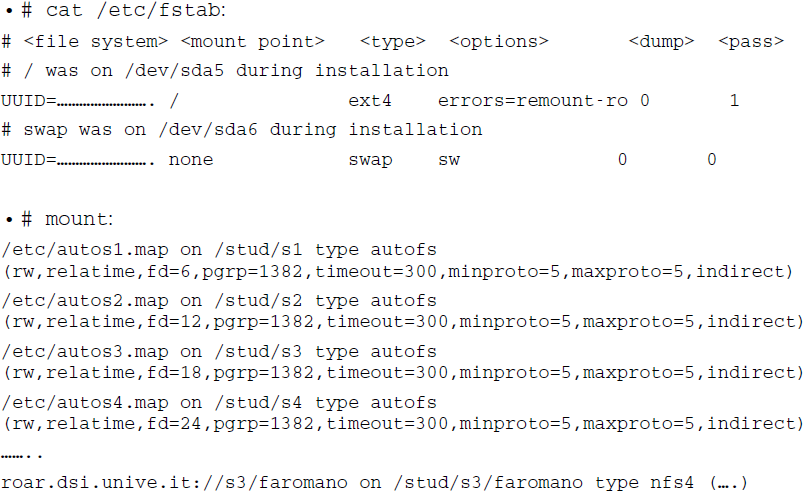
\includegraphics[scale=0.6]{autofslab.png}
\end{center}
\paragraph{CIFS} Prima di proseguire, è importante definire il concetto di \textbf{Roaming User Profile}: si tratta di un concetto chiave nella famiglia di sistemi operativi Windows NT, in quanto permette a ogni utente con un computer collegato a un dominio Windows Server di effettuare il login su qualunque computer nello stesso network e accedere ai suoi documenti, applicazioni, ecc.. Questo concetto è diverso dalle home esportate, in quanto queste sono cartelle condivise presenti in \texttt{Z} da usare per salvare i files importanti.\\
Va tenuto conto che i profili sono in una cartella condivisa, ma vengono scaricati e caricati dal server ogni volta che fate login e logout rispettivamente: non sono live, e fanno spesso fatica a sincronizzarsi.\\
In Windows, la condivisione dei files è gestita dal protocollo CIFS, di cui esiste un'implementazione in Linux di nome SAMBA.\\
CIFS è un protocollo standard che permette la condivisione di files e risorse all'interno di una LAN. È una versione migliorata del protocollo Microsoft SMB, e nasce con Windows 2000 come unico protocollo di condivisione risorse.\\
Nonostante molte migliorie, resta ancora inefficiente in reti di medie/grosse dimensioni. Ma è comunque uno dei migliori protocolli per una realizzazione di DFS.\\
Dal punto di vista tecnico, CIFS permette l'accesso multiplo allo stesso file evitando conflitti tramite file locking, è ottimizzato per le connessioni lente, supporta sia il trasferimento dei file anonimo sia previa autenticazione, è scalabile, supporta varie codifiche dei caratteri, e per riferirsi a un file remoto non devono necessariamente montare il FS remoto ma possono usare un path UNC (Uniform Naming Convention, es.: \texttt{\textbackslash\textbackslash nas\textbackslash bustepaga\textbackslash pagamiseradisettembre.pdf}).\\
Per condividere una cartella o un file, cliccateci col tasto destro, scegliete "condividi", impostate i permessi, e alla fine sulla barra degli indirizzi del file explorer digitate\\
\tab\texttt{\textbackslash\textbackslash server\textbackslash cartellaappenacondivisa}\\
CIFS ha un problema non indifferente. In un ambiente multiutente, spesso vi è competizione tra gli utenti stessi per l'uso delle risorse. Una delle più importanti, poiché l'uso non è limitato al periodo in cui l'utente sta effettivamente operando sulla macchina, è lo spazio di memorizzazione. Questo spazio, per ragioni di presentazioni, affidabilità e disponibilità continua, è generalmente molto più costoso di quanto lo sia l'equivalente nell'ambito dei personal computer. \\
Diventa necessario proteggere il sistema e gli altri utenti da chi vuole monopolizzare la risorsa sia volontariamente, che involontariamente (programmi errati che esauriscono lo spazio del disco) in quanto una volta terminato lo spazio sul disco, nessun utente può lavorare.\\
Per far fronte a questo problema, è stato introdotto il concetto di \textbf{quota disco}: un limite oltre al quale uno specifico utente non può più occupare spazio.\\
La quota può essere usata anche su FS locali, ma trova la sua più naturale applicazione quando le home directory (o altri dati personali) degli utenti vengono condivise tramite NAS. In Linux il sistema di quota viene gestito direttamente dal Kernel, mentre le utilities per la gestione sono presenti nel pacchetto \texttt{quota}.\\
La quota, se presente, viene automaticamente usata anche per le operazioni sui FS esportati, tuttavia se si vuole poter conoscere le informazioni sulla quota disponibile (con il comando \texttt{quota}) anche sui client, è necessario usare il daemon \texttt{rquotad}.\\
La quota è espressa in quattro quantità:
\begin{itemize}
\item Soft quota sul numero di blocchi, al suo raggiungimento si ottiene un warning.
\item Hard quota sul numero di blocchi, al suo raggiungimento viene negata ogni richiesta di allocazione.
\item Soft quota sugli inode, ovvero un warning quando vengono creati un certo numero di files o directories.
\item Hard quota sugli inode, ovvero alla creazione di un certo numero di files o directories viene negata ogni creazione successiva.
\end{itemize}
Per entrambe le soft quota, inoltre, esiste il \textbf{grace period}. Se oltre questo periodo l'utente si mantiene sopra la soglia della soft quota, ogni altra allocazione/creazione di file o directory verrà negata.\\
Per installare il pacchetto \texttt{quota} si usa il comando\\
\tab\texttt{apt-get install quota}\\
Supponiamo di voler mettere la quota su \texttt{/user}. Editiamo il file \texttt{/etc/fstab}, abilitando la quota sulla riga corrispondente al FS \texttt{/user}:\\
\tab\texttt{/dev/sda5\tab /user\tab ext4\tab usrquota,grpquota\tab 0 1}\\
Rimontiamo \texttt{/user} abilitando le quote:\\
\tab\texttt{mount -o remount /user}\\
Dopodiché, eseguiamo il comando\\
\tab\texttt{quotacheck -cu /user /* c:crea, u:user, (g:group) */}\\
Questo comando crea un nuovo file delle quote nella directory principale del FS. Questo è un file indicizzato utilizzato dallo strumento per la gestione della quota per tenere traccia dello spazio disco usato dall'utente. Esso contiene anche i limiti per gli utenti e le opzioni configurate.\\
Abilitiamo la quota col comando\\
\tab\texttt{quotaon /user}\\
A questo punto abbiamo un sistema di quota sulla partizione \texttt{/user} che potete gestire con i comandi \texttt{edquota}, \texttt{setquota} e \texttt{repquota}.\\
\chapter{Web}
\paragraph{World Wide Web (WWW)} è il sistema che permette la condivisione di documenti ipertestuali multimediali, costituiti cioè da un insieme di contenuti testuali, visuali e audio/video, sfruttando l'infrastruttura di internet.\\
Il Web nasce come sistema di gestione di ipertesti in ambiente distribuito, per poi assumere i ruoli più svariati: dal veicolo di contenuti e flussi multimediali, all'interfaccia per applicazione interattive. Viene sviluppato al CERN nel 1989 per poi venire "regalato" al pubblico nel 1991. Si basa sul protocollo HTTP, ha un'architettura di tipo client/server ed è il servizio più diffuso di internet.\\
La prima versione del protocollo HTTP prevedeva che in una sessione il client (browser) potesse fare una singola richiesta di una risorsa (un pathname) al server, e che quest'ultimo potesse solo rispondere a tali richieste.\\
Il protocollo HTTP 1.1 introdusse la possibilità di avere più richieste per connessione, di avere connessioni permanenti e, all'interno di queste, di mandare richieste/risposte asincrone.\\
Il protocollo obbliga inoltre i client a specificare, nella richiesta, qual è l'hostname dal quale si vuole ottenere una risorsa. Questo permette di implementare il virtual hosting, in cui un server può ospitare più siti internet raggiungibili utsando nomi diversi, sebbene corrispondano sempre allo stesso IP.\\
Il \textbf{Web server} è un'applicazione software che, in esecuzione su un \textbf{host server}, è in grado di gestire le richieste di trasferimento di pagine web di un client, di solito web browser. La comunicazione tra server e client avviene tramite il protocollo HTTP che utilizza la porta TCP 80, o eventualmente HTTPS che utilizza la 443.\\
Tutti i web server forniscono pagine web standard allo stesso modo: in sostanza, tutti gestiscono richieste HTML e CSS. L'interpretazione del codice inviato è fatta dal browser, ma ognuno di essi ha delle peculiarità che permettono di gestire applicazioni dinamiche diverse.\\
Elenco di Web Servers:
\begin{itemize}
\item \textbf{NCSA HTTP:} il più diffuso prima di Apache.
\item \textbf{Apache HTTP Server:} sviluppato da Apache Software Foundation, è il più diffuso, ed è l'unico che grazie ad una tecnologia modulare è in grado di gestire applicazioni di tutti i tipi: php, python, java, ecc..
\item \textbf{Apache Tomcat:} sviluppato anch'esso da Apache Software Foundation, fornisce un sistema di gestione delle servlet java.
\item \textbf{Light HTTPD}
\item \textbf{Ngix}
\item \textbf{Internet Information Services (IIS):} sviluppato da Microsoft, permette la gestione di applicazioni .NET, nelle nuove versioni è stato gradualmente introdotto il supporto per PHP.
\end{itemize}
\begin{center}
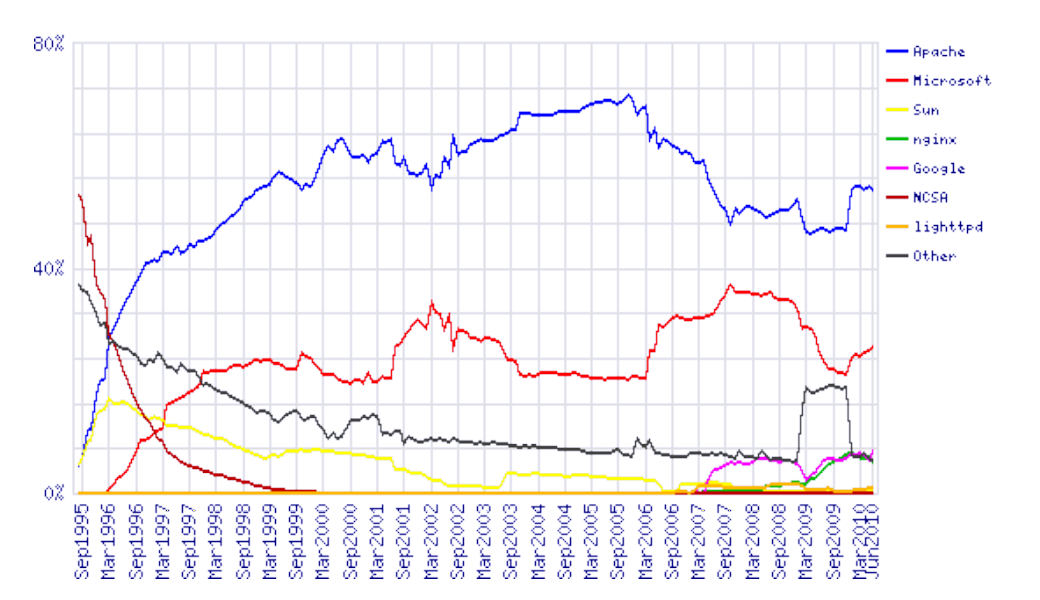
\includegraphics[scale=0.5]{diffusioneweb.png}
\end{center}
\paragraph{Apache HTTP Server} È il server web modulare più diffuso, in grado di operare su una grande varietà di sistemi operativi, tra cui UNIX/Linux, Microsoft Windows e OS X.\\
L'architettura è composta da un daemon (servizio) che, sulla base delle impostazioni contenute nel file di configurazione \texttt{httpd.conf}, permette l'accesso a uno o più siti, gestendo varie caratteristiche di sicurezza e potendo ospitare diverse estensioni per pagine attive (o dinamiche), come PHP o Jakarta/Tomcat.\\
Il Web Server Apache presenta un'architettura modulare, quindi a ogni richiesta del client vengono svolte funzioni specifiche da ogni modulo di cui è composto, come unità indipendenti. Ciascun modulo si occupa di una funzionalità, e il controllo è gestito dal core.\\
Il core è sostanzialmente un daemon che esegue un ciclo di polling, attraverso il quale vengono interrogate continuamente le linee logiche da cui possono pervenire messaggi di richiesta. Il core provvede al passaggio della richiesta ai vari moduli in modo sequenziale, usando i parametri di uscita di un modulo come parametri di accesso per il successivo, creando così l'illusione di una comunicazione orizzontale fra moduli.\\
\begin{center}
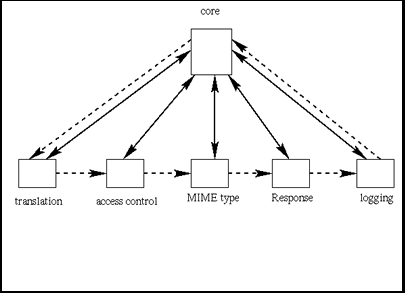
\includegraphics[scale=0.7]{core.png}
\end{center}
Esempio di installazione si LAMP Server su Ubuntu:\\
\tab\texttt{\# apt-get install lamp-server\^}\tab metapacchetto\\
\tab\texttt{\# apt-get install phpmyadmin}\\
Al termine dell'installazione abbiamo a disposizione un web server Apache 2, un database server MySQL, PHP 5 con il modulo per Apache e la libreria \texttt{gd} e phpMyAdmin per la gestione dei database.\\
Apache normalmente va a leggere i files che compongono il sito nella cartella \texttt{/var/www}. Questa posizione viene definita \texttt{DocumentRoot}, e può essere cambiata. Tutti i files di configurazione di Apache risiedono in \texttt{/etc/apache2}.\\
In particolare:
\begin{itemize}
\item \textbf{apache2.conf:} file con la configurazione iniziale di Apache.
\item \textbf{ports.conf:} specifica le porte di ascolto del demone Apache.
\item \textbf{conf-available:} configurazioni aggiuntive disponibili.
\item \textbf{conf-enabled:} configurazioni aggiuntive attive.
\item \textbf{mods-available:} moduli disponibili.
\item \textbf{mods-enabled:} moduli attivi.
\item \textbf{sites-available:} siti disponibili.
\item \textbf{sites-enabled:} siti attivi.
\end{itemize}
Se create una pagina HTML e la copiate in \texttt{/var/www} potete puntare il browser verso \texttt{http://myserver.mydomain/mypage.html}. Se puntate il browser su \texttt{http://myserver.mydomain/phpmyadmin} trovate l'interfaccia di gestione di mysql.\\
\paragraph{VirtualHost:} permette a un server web di ospitare più di un dominio. Utile in ambienti condivisi di web hosting poiché permette di collocare centinaia di siti web in un unico server fisico. Implementato anche nei moderni software di web server: Apache, Nginx, IIS, Lighttpd. In Apache è implementato dalla direttiva \texttt{VirtualHost}.\\
Un esempio di VirtualHost è dato dal server \texttt{www} del DAIS, che ospita svariati siti web. Un esempio di questi è un progetto denominato \texttt{sanitaveneto}. Si vuole che il server Web risponda alle richieste per \texttt{sanitaveneto.dais.unive.it} e \texttt{sanitaveneto.ds.unive.it}.\\
Anzitutto è necessario definire una entry nel server DNS che faccia puntare \texttt{sanitaveneto} al server \texttt{www}:\\
\tab\texttt{Sanitaveneto A 157.138.20.11}\tab (in questo caso bisogna inserire\tab anche il reverse)\\
Oppure\\
\tab\texttt{sanitaveneto CNAME www}\\
Successivamente bisogna creare la directory dove il sito sarà ospitato e i relativi files di log:\\
\tab\texttt{\# mkdir /var/www/sanitaveneto}\\
\tab\texttt{\# mkdir /var/log/apache2/sanitaveneto}\\
Ricordiamoci di dare gli accessi alla directory del sito all'utente \texttt{www-data}:\\
\tab\texttt{\# chown -R www-data:www-data /var/www/sanitaveneto}\\
Creiamo il file di configurazione del VirtualHost:\\
\tab\texttt{\# nano /etc/apache2/sites-available/sanitaveneto}\\
E inseriamo il seguente testo:\\
\tab\texttt{<VirtualHost *:80>}\\
\tab\tab\texttt{ServerAdmin webmaster@dsi.unive.it}\\
\tab\tab\texttt{ServerName sanitaveneto.dais.unive.it}\\
\tab\tab\texttt{DocumentRoot /var/www/sanitaveneto/}\\
\tab\tab\texttt{ErrorLog /var/log/apache2/sanitaveneto.error.log}\\
\tab\tab\texttt{LogLevel warn}\\
\tab\tab\texttt{CustomLog /var/log/apache2/sanitaveneto.access.log combined}\\
\tab\tab\texttt{ServerSignature Off}\\
\tab\texttt{</VirtualHost>}\\
Ora non resta che attivare il sito e riavviare apache:\\
\tab\texttt{\# a2ensite sanitaveneto.conf}\\
\tab\texttt{\# service apache2 restart}\\
Comandi utili di Apache:
\begin{itemize}
\item \texttt{\# a2ensite <nomesito>} abilita un sito web presente
in sites-avaiable.
\item \texttt{\# a2dissite <nomesito>} disabilita un sito web
presente in sites-enabled.
\item \texttt{\# a2enmod <modulo>} abilita un modulo di apache
disponibile in mods-avaiable.
\item \texttt{\# a2dismod <modulo>} disabilita un modulo di apache.
\item \texttt{\# ab} apache benchmark.
\item \texttt{\# service apache <start|restart|stop>} per avviare, riavviare e fermare un servizio.
\end{itemize}
\begin{center}
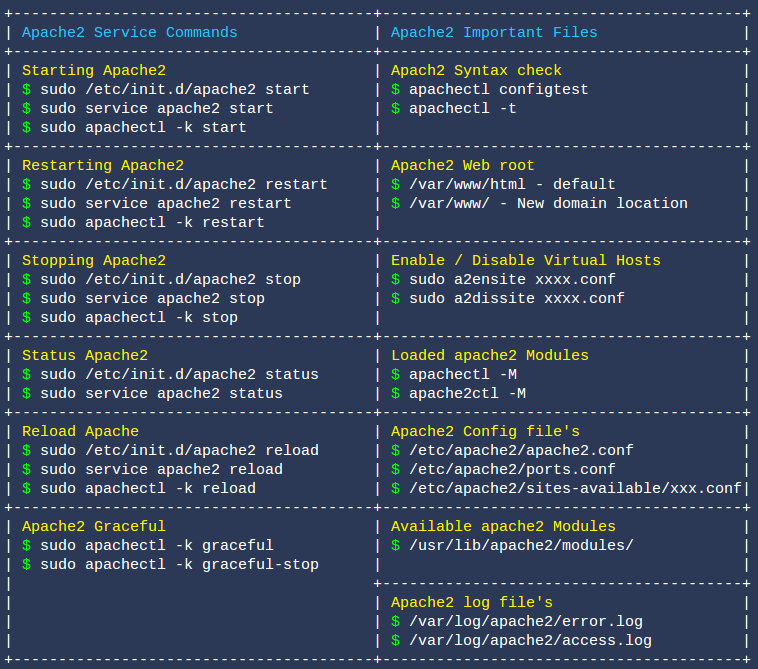
\includegraphics[scale=0.6]{comandiapache.png}
\end{center}
\paragraph{SSL} La crittografia è importante per la sicurezza, deve essere usata in tutte quelle applicazioni che richiedono autenticazione (come un form web) e che trasmettono dati sensibili. Non protegge completamente da attacchi informatici, ma complica il lavoro a chi nutre cattive intenzioni. La crittografia può anche essere utilizzata per attaccare gli utenti, come nel caso del \texttt{ransomware} WannaCry.\\
\textbf{Transport Layer Security (TLS)} e il suo predecessore \textbf{Secure Sockets Layer (SSL)} sono dei protocolli crittografici usati nel campo delle telecomunicazioni e dell'informatica che permettono una comunicazione sicura dal sorgente al destinatario (end-to-end) su reti TCP/IP fornendo un'autenticazione, integrità dei dati e cifratura operando al di sopra del livello di trasporto.\\
Esempi di applicazione di SSL/TLS sono nei protocolli HTTPS, SMTPS, POP3S, IMAPS, ecc..\\
Vi sono varie implementazioni di SSL, quella più famosa è probabilmente OpenSSL, implementata per tutti i sistemi Linux.\\
\paragraph{OpenSSL} Nato nel 1998, il progetto \textbf{OpenSSL} è un'implementazione open source del protocollo SSL/TLS. La libreria principale è scritta in linguaggio C e implementa funzioni di crittografia basilari fornendo strumenti per l'attivazione di varie funzionalità avanzate. Ne esistono versioni per la gran parte dei sistemi operativi UNIX (Solaris, Linux, OS X e alcune versioni open source di BSD) e Microsoft Windows. Ideato come un set di strumenti aperto per la crittografia del codice e dello scambio di dati che avviene su Internet, oggi è utilizzato da circa il 3/4 dei server della Rete.\\
OpenSSL ha conquistato, suo malgrado, l'attenzione della stampa internazionale a causa di una sua falla di sicurezza sfruttata dall'attacco Heartbleed.\\
OpenSSL permette di utilizzare sia certificati rilasciati da certification authorities valide, sia autogenerati (in questo caso i browser avvertiranno l'utente che il certificato può non essere sicuro).\\
Un esempio di uso di OpenSSL è la combinazione di Apache e SSL, che risulta in HTTPS: un protocollo simile ad HTTP che permette connessione crittografate per garantire la sicurezza dei dati. Un server HTTPS si può realizzare tramite il modulo SSL di Apache e risponderà sulla porta 443.\\
Ora proporremo un esempio facendo finta di aver già generato un certificato SSL.\\
Attiviamo il modulo SSL e riavviamo Apache:\\
\tab\texttt{\# a2enmod ssl \&\& service apache2 restart}\\
Creiamo una directory dove mettere il certificato appena generato:\\
\tab\texttt{\# mkdir /etc/apache/ssl}\\
Creiamo il certificato:\\
\tab\texttt{\# sudo openssl req -x509 -nodes -days 3650 -newkey rsa:2048}\\
\tab\texttt{-keyout /etc/apache2/ssl/apache.key -out /etc/apache2/ssl/apache.crt}\\
Configuriamo ora Apache creando un nuovo sito:\\
\tab\texttt{\# nano /etc/apache2/sites-available/default-ssl.conf}\\
E vi inseriamo la configurazione:\\
\texttt{
\tab <IfModule mod\_ssl.c>\\
\tab\tab Listen: 443\\
\tab\tab <VirtualHost \_default\_:443>\\
\tab\tab\tab ServerAdmin webmaster@mydomain\\
\tab\tab\tab ServerName myhttps.mydomain\\
\tab\tab\tab ServerAlias www.myhttps.mydomain\\
\tab\tab\tab DocumentRoot /var/www/html\\
\tab\tab\tab ErrorLog \$\{APACHE\_LOG\_DIR\}/error.log\\
\tab\tab\tab CustomLog \$\{APACHE\_LOG\_DIR\}/access.log combined\\
\tab\tab\tab SSLEngine on\\
\tab\tab\tab SSLCertificateFile /etc/apache2/ssl/apache.crt\\
\tab\tab\tab SSLCertificateKeyFile /etc/apache2/ssl/apache.key\\
\tab\tab\tab BrowserMatch "MSIE [26]"\textbackslash\\
\tab\tab\tab\tab nokeepalive ssl-unclean-shutdown\textbackslash\\
\tab\tab\tab\tab downgrade-1.0 force-response-1.0\\
\tab\tab\tab BrowserMatch "MSIE [179]" ssl-unclean-shutdown\\
\tab\tab</VirtualHost>\\
\tab</IfModule>\\
}\\
Abilitiamo il sito:\\
\tab\texttt{\# a2ensite default-ssl.conf}\\
Riavviamo apache:\\
\tab\texttt{\# service apache2 restart}\\
A questo punto puntiamo il server verso \texttt{https://myporta.mydomain/mypage.html} e dovremo vedere il nostro sito protetto con SSL.\\
Un esempio dell'uso di apache sono i sistemi di monitoring.\\
\paragraph{Sistemi di monitoring} 
\begin{itemize}
\item \textbf{Sistemi di basso livello:} controllo dello stato di salute dei dischi, controllo dello stato del RAID, controllo delle memorie ECC, sensori di temperatura, indicatori di velocità delle ventole, ecc..
\item \textbf{Sistemi a livello SO:} Lm-sensors, hddtemp, smartd che controllano i sistemi di basso livello, watchdog che controlla errori del sistema operativo.
\end{itemize}
Ad un livello più alto troviamo i software di monitoring e di raccolta dati del sistema:
\begin{itemize}
\item \textbf{Nagios:} permette di controllare un grande numero di host, monitorando hardware e software dei vari host e lo stato dei servizi ospitati.
\item \textbf{Mrtg, mailgraph, cacti, ganglia:} raccolgono statistiche e le interpretano sotto forma di grafici per descrivere l'uso del sistema.
\end{itemize}
I software sopracitati possono acquisire i dati da una varietà di fonti eterogenee, spesso usando metodi ad-hoc. Esiste tuttavia un protocollo per il monitoring dei dispositivi, il Simple Network Management Protocol (SNMP).












\end{document}